
%% bare_conf.tex
%% V1.3
%% 2007/01/11
%% by Michael Shell
%% See:
%% http://www.michaelshell.org/
%% for current contact information.
%%
%% This is a skeleton file demonstrating the use of IEEEtran.cls
%% (requires IEEEtran.cls version 1.7 or later) with an IEEE conference paper.
%%
%% Support sites:
%% http://www.michaelshell.org/tex/ieeetran/
%% http://www.ctan.org/tex-archive/macros/latex/contrib/IEEEtran/
%% and
%% http://www.ieee.org/

%%*************************************************************************
%% Legal Notice:
%% This code is offered as-is without any warranty either expressed or
%% implied; without even the implied warranty of MERCHANTABILITY or
%% FITNESS FOR A PARTICULAR PURPOSE! 
%% User assumes all risk.
%% In no event shall IEEE or any contributor to this code be liable for
%% any damages or losses, including, but not limited to, incidental,
%% consequential, or any other damages, resulting from the use or misuse
%% of any information contained here.
%%
%% All comments are the opinions of their respective authors and are not
%% necessarily endorsed by the IEEE.
%%
%% This work is distributed under the LaTeX Project Public License (LPPL)
%% ( http://www.latex-project.org/ ) version 1.3, and may be freely used,
%% distributed and modified. A copy of the LPPL, version 1.3, is included
%% in the base LaTeX documentation of all distributions of LaTeX released
%% 2003/12/01 or later.
%% Retain all contribution notices and credits.
%% ** Modified files should be clearly indicated as such, including  **
%% ** renaming them and changing author support contact information. **
%%
%% File list of work: IEEEtran.cls, IEEEtran_HOWTO.pdf, bare_adv.tex,
%%                    bare_conf.tex, bare_jrnl.tex, bare_jrnl_compsoc.tex
%%*************************************************************************

% *** Authors should verify (and, if needed, correct) their LaTeX system  ***
% *** with the testflow diagnostic prior to trusting their LaTeX platform ***
% *** with production work. IEEE's font choices can trigger bugs that do  ***
% *** not appear when using other class files.                            ***
% The testflow support page is at:
% http://www.michaelshell.org/tex/testflow/



% Note that the a4paper option is mainly intended so that authors in
% countries using A4 can easily print to A4 and see how their papers will
% look in print - the typesetting of the document will not typically be
% affected with changes in paper size (but the bottom and side margins will).
% Use the testflow package mentioned above to verify correct handling of
% both paper sizes by the user's LaTeX system.
%
% Also note that the "draftcls" or "draftclsnofoot", not "draft", option
% should be used if it is desired that the figures are to be displayed in
% draft mode.
%
\documentclass[conference]{IEEEtran}
% Add the compsoc option for Computer Society conferences.
%
% If IEEEtran.cls has not been installed into the LaTeX system files,
% manually specify the path to it like:
% \documentclass[conference]{../sty/IEEEtran}





% Some very useful LaTeX packages include:
% (uncomment the ones you want to load)


% *** MISC UTILITY PACKAGES ***
%
%\usepackage{ifpdf}
% Heiko Oberdiek's ifpdf.sty is very useful if you need conditional
% compilation based on whether the output is pdf or dvi.
% usage:
% \ifpdf
%   % pdf code
% \else
%   % dvi code
% \fi
% The latest version of ifpdf.sty can be obtained from:
% http://www.ctan.org/tex-archive/macros/latex/contrib/oberdiek/
% Also, note that IEEEtran.cls V1.7 and later provides a builtin
% \ifCLASSINFOpdf conditional that works the same way.
% When switching from latex to pdflatex and vice-versa, the compiler may
% have to be run twice to clear warning/error messages.






% *** CITATION PACKAGES ***
%
\usepackage{cite}
% cite.sty was written by Donald Arseneau
% V1.6 and later of IEEEtran pre-defines the format of the cite.sty package
% \cite{} output to follow that of IEEE. Loading the cite package will
% result in citation numbers being automatically sorted and properly
% "compressed/ranged". e.g., [1], [9], [2], [7], [5], [6] without using
% cite.sty will become [1], [2], [5]--[7], [9] using cite.sty. cite.sty's
% \cite will automatically add leading space, if needed. Use cite.sty's
% noadjust option (cite.sty V3.8 and later) if you want to turn this off.
% cite.sty is already installed on most LaTeX systems. Be sure and use
% version 4.0 (2003-05-27) and later if using hyperref.sty. cite.sty does
% not currently provide for hyperlinked citations.
% The latest version can be obtained at:
% http://www.ctan.org/tex-archive/macros/latex/contrib/cite/
% The documentation is contained in the cite.sty file itself.



\usepackage{graphicx}


% *** GRAPHICS RELATED PACKAGES ***
%
\ifCLASSINFOpdf
  % \usepackage[pdftex]{graphicx}
  % declare the path(s) where your graphic files are
  % \graphicspath{{../pdf/}{../jpeg/}}
  % and their extensions so you won't have to specify these with
  % every instance of \includegraphics
  % \DeclareGraphicsExtensions{.pdf,.jpeg,.png}
\else
  % or other class option (dvipsone, dvipdf, if not using dvips). graphicx
  % will default to the driver specified in the system graphics.cfg if no
  % driver is specified.
  % \usepackage[dvips]{graphicx}
  % declare the path(s) where your graphic files are
  % \graphicspath{{../eps/}}
  % and their extensions so you won't have to specify these with
  % every instance of \includegraphics
  % \DeclareGraphicsExtensions{.eps}
\fi
% graphicx was written by David Carlisle and Sebastian Rahtz. It is
% required if you want graphics, photos, etc. graphicx.sty is already
% installed on most LaTeX systems. The latest version and documentation can
% be obtained at: 
% http://www.ctan.org/tex-archive/macros/latex/required/graphics/
% Another good source of documentation is "Using Imported Graphics in
% LaTeX2e" by Keith Reckdahl which can be found as epslatex.ps or
% epslatex.pdf at: http://www.ctan.org/tex-archive/info/
%
% latex, and pdflatex in dvi mode, support graphics in encapsulated
% postscript (.eps) format. pdflatex in pdf mode supports graphics
% in .pdf, .jpeg, .png and .mps (metapost) formats. Users should ensure
% that all non-photo figures use a vector format (.eps, .pdf, .mps) and
% not a bitmapped formats (.jpeg, .png). IEEE frowns on bitmapped formats
% which can result in "jaggedy"/blurry rendering of lines and letters as
% well as large increases in file sizes.
%
% You can find documentation about the pdfTeX application at:
% http://www.tug.org/applications/pdftex





% *** MATH PACKAGES ***
%
\usepackage[cmex10]{amsmath}
% A popular package from the American Mathematical Society that provides
% many useful and powerful commands for dealing with mathematics. If using
% it, be sure to load this package with the cmex10 option to ensure that
% only type 1 fonts will utilized at all point sizes. Without this option,
% it is possible that some math symbols, particularly those within
% footnotes, will be rendered in bitmap form which will result in a
% document that can not be IEEE Xplore compliant!
%
% Also, note that the amsmath package sets \interdisplaylinepenalty to 10000
% thus preventing page breaks from occurring within multiline equations. Use:
%\interdisplaylinepenalty=2500
% after loading amsmath to restore such page breaks as IEEEtran.cls normally
% does. amsmath.sty is already installed on most LaTeX systems. The latest
% version and documentation can be obtained at:
% http://www.ctan.org/tex-archive/macros/latex/required/amslatex/math/





% *** SPECIALIZED LIST PACKAGES ***
%
%\usepackage{algorithmic}
% algorithmic.sty was written by Peter Williams and Rogerio Brito.
% This package provides an algorithmic environment fo describing algorithms.
% You can use the algorithmic environment in-text or within a figure
% environment to provide for a floating algorithm. Do NOT use the algorithm
% floating environment provided by algorithm.sty (by the same authors) or
% algorithm2e.sty (by Christophe Fiorio) as IEEE does not use dedicated
% algorithm float types and packages that provide these will not provide
% correct IEEE style captions. The latest version and documentation of
% algorithmic.sty can be obtained at:
% http://www.ctan.org/tex-archive/macros/latex/contrib/algorithms/
% There is also a support site at:
% http://algorithms.berlios.de/index.html
% Also of interest may be the (relatively newer and more customizable)
% algorithmicx.sty package by Szasz Janos:
% http://www.ctan.org/tex-archive/macros/latex/contrib/algorithmicx/




% *** ALIGNMENT PACKAGES ***
%
%
\usepackage{array}
% Frank Mittelbach's and David Carlisle's array.sty patches and improves
% the standard LaTeX2e array and tabular environments to provide better
% appearance and additional user controls. As the default LaTeX2e table
% generation code is lacking to the point of almost being broken with
% respect to the quality of the end results, all users are strongly
% advised to use an enhanced (at the very least that provided by array.sty)
% set of table tools. array.sty is already installed on most systems. The
% latest version and documentation can be obtained at:
% http://www.ctan.org/tex-archive/macros/latex/required/tools/


%\usepackage{mdwmath}
%\usepackage{mdwtab}
% Also highly recommended is Mark Wooding's extremely powerful MDW tools,
% especially mdwmath.sty and mdwtab.sty which are used to format equations
% and tables, respectively. The MDWtools set is already installed on most
% LaTeX systems. The lastest version and documentation is available at:
% http://www.ctan.org/tex-archive/macros/latex/contrib/mdwtools/


% IEEEtran contains the IEEEeqnarray family of commands that can be used to
% generate multiline equations as well as matrices, tables, etc., of high
% quality.


\usepackage{eqparbox}
% Also of notable interest is Scott Pakin's eqparbox package for creating
% (automatically sized) equal width boxes - aka "natural width parboxes".
% Available at:
% http://www.ctan.org/tex-archive/macros/latex/contrib/eqparbox/





% *** SUBFIGURE PACKAGES ***
%\usepackage[tight,footnotesize]{subfigure}
% subfigure.sty was written by Steven Douglas Cochran. This package makes it
% easy to put subfigures in your figures. e.g., "Figure 1a and 1b". For IEEE
% work, it is a good idea to load it with the tight package option to reduce
% the amount of white space around the subfigures. subfigure.sty is already
% installed on most LaTeX systems. The latest version and documentation can
% be obtained at:
% http://www.ctan.org/tex-archive/obsolete/macros/latex/contrib/subfigure/
% subfigure.sty has been superceeded by subfig.sty.



%\usepackage[caption=false]{caption}
%\usepackage[font=footnotesize]{subfig}
% subfig.sty, also written by Steven Douglas Cochran, is the modern
% replacement for subfigure.sty. However, subfig.sty requires and
% automatically loads Axel Sommerfeldt's caption.sty which will override
% IEEEtran.cls handling of captions and this will result in nonIEEE style
% figure/table captions. To prevent this problem, be sure and preload
% caption.sty with its "caption=false" package option. This is will preserve
% IEEEtran.cls handing of captions. Version 1.3 (2005/06/28) and later 
% (recommended due to many improvements over 1.2) of subfig.sty supports
% the caption=false option directly:
%\usepackage[caption=false,font=footnotesize]{subfig}
%
% The latest version and documentation can be obtained at:
% http://www.ctan.org/tex-archive/macros/latex/contrib/subfig/
% The latest version and documentation of caption.sty can be obtained at:
% http://www.ctan.org/tex-archive/macros/latex/contrib/caption/




% *** FLOAT PACKAGES ***
%
%\usepackage{fixltx2e}
% fixltx2e, the successor to the earlier fix2col.sty, was written by
% Frank Mittelbach and David Carlisle. This package corrects a few problems
% in the LaTeX2e kernel, the most notable of which is that in current
% LaTeX2e releases, the ordering of single and double column floats is not
% guaranteed to be preserved. Thus, an unpatched LaTeX2e can allow a
% single column figure to be placed prior to an earlier double column
% figure. The latest version and documentation can be found at:
% http://www.ctan.org/tex-archive/macros/latex/base/



%\usepackage{stfloats}
% stfloats.sty was written by Sigitas Tolusis. This package gives LaTeX2e
% the ability to do double column floats at the bottom of the page as well
% as the top. (e.g., "\begin{figure*}[!b]" is not normally possible in
% LaTeX2e). It also provides a command:
%\fnbelowfloat
% to enable the placement of footnotes below bottom floats (the standard
% LaTeX2e kernel puts them above bottom floats). This is an invasive package
% which rewrites many portions of the LaTeX2e float routines. It may not work
% with other packages that modify the LaTeX2e float routines. The latest
% version and documentation can be obtained at:
% http://www.ctan.org/tex-archive/macros/latex/contrib/sttools/
% Documentation is contained in the stfloats.sty comments as well as in the
% presfull.pdf file. Do not use the stfloats baselinefloat ability as IEEE
% does not allow \baselineskip to stretch. Authors submitting work to the
% IEEE should note that IEEE rarely uses double column equations and
% that authors should try to avoid such use. Do not be tempted to use the
% cuted.sty or midfloat.sty packages (also by Sigitas Tolusis) as IEEE does
% not format its papers in such ways.





% *** PDF, URL AND HYPERLINK PACKAGES ***
%
\usepackage{url}
% url.sty was written by Donald Arseneau. It provides better support for
% handling and breaking URLs. url.sty is already installed on most LaTeX
% systems. The latest version can be obtained at:
% http://www.ctan.org/tex-archive/macros/latex/contrib/misc/
% Read the url.sty source comments for usage information. Basically,
% \url{my_url_here}.
\usepackage[utf8]{inputenc}




% *** Do not adjust lengths that control margins, column widths, etc. ***
% *** Do not use packages that alter fonts (such as pslatex).         ***
% There should be no need to do such things with IEEEtran.cls V1.6 and later.
% (Unless specifically asked to do so by the journal or conference you plan
% to submit to, of course. )


% correct bad hyphenation here
\hyphenation{op-tical net-works semi-conduc-tor}


\begin{document}
%
% paper title
% can use linebreaks \\ within to get better formatting as desired
\title{Analysis of the design pattern Model View Presenter on the Android platform using OO quality metrics}


% author names and affiliations
% use a multiple column layout for up to three different
% affiliations
\author{\IEEEauthorblockN{Diego L. Freitas}
\IEEEauthorblockA{Departamento de Software e Hardware\\
Fundação Desembargador Paulo Feitoza (FPF-Tech)\\
Manaus, Brazil\\
Email: diego.freitas@fpf.br}
\and
\IEEEauthorblockN{Danny Lopes}
\IEEEauthorblockA{FUCAPI - Departamento de Tecnologia\\
Manaus, Brazil\\
Email: danny.lopes@fucapi.br}
}

% conference papers do not typically use \thanks and this command
% is locked out in conference mode. If really needed, such as for
% the acknowledgment of grants, issue a \IEEEoverridecommandlockouts
% after \documentclass

% for over three affiliations, or if they all won't fit within the width
% of the page, use this alternative format:
% 
%\author{\IEEEauthorblockN{Michael Shell\IEEEauthorrefmark{1},
%Homer Simpson\IEEEauthorrefmark{2},
%James Kirk\IEEEauthorrefmark{3}, 
%Montgomery Scott\IEEEauthorrefmark{3} and
%Eldon Tyrell\IEEEauthorrefmark{4}}
%\IEEEauthorblockA{\IEEEauthorrefmark{1}School of Electrical and Computer Engineering\\
%Georgia Institute of Technology,
%Atlanta, Georgia 30332--0250\\ Email: see http://www.michaelshell.org/contact.html}
%\IEEEauthorblockA{\IEEEauthorrefmark{2}Twentieth Century Fox, Springfield, USA\\
%Email: homer@thesimpsons.com}
%\IEEEauthorblockA{\IEEEauthorrefmark{3}Starfleet Academy, San Francisco, California 96678-2391\\
%Telephone: (800) 555--1212, Fax: (888) 555--1212}
%\IEEEauthorblockA{\IEEEauthorrefmark{4}Tyrell Inc., 123 Replicant Street, Los Angeles, California 90210--4321}}




% use for special paper notices
%\IEEEspecialpapernotice{(Invited Paper)}




% make the title area
\maketitle


\begin{abstract}

The Android platform has been adopted by several vendors of smartphones and
tablets promoting a comprehensive dissemination of the operating system.
Formed a large market to be exploited for application delivery
for the most varied purposes. To meet this demand is necessary to
develop applications with good quality at a high level of productivity.
However, for dealing with applications designed to meet specific needs and with a
short development cycle, there is little concern with the architecture of
solution, resulting in products with poor quality. Within the engineering
there are software design patterns that help in the development of software.
This work aims to present the application of the design pattern
Model View Presenter in android application development to increase
application quality. The effects that this pattern has on the object of study
are assessed on an object-oriented perspective. The experimental method is
iteratively applied using the process of incremental refactoring
collecting quality metrics of code to do a quantitative analysis.
The results show that the application of the design pattern increased the
cohesion of the code, however, with a small increase in complexity due to the
inclusion of new components used to divide responsibilities.


\noindent
\textbf{Keywords}: Android. Model View Presenter. Design Patterns.

\end{abstract}

\section{Introdução}

Segundo \cite{idc} o mercado de dispositivos móveis ultrapassou a marca de mais de um
bilhão de aparelhos vendidos em 2013. A plataforma Android é a líder
de mercado dominando 78\% desse universo com mais de 226.1 milhões de
Smartphones produzidos e embarcados com android no último quadrimestre de 2013.
Baseado nesses dados é possível concluir que existe uma demanda latente no
desenvolvimento de novos aplicativos que agreguem valor à esta plataforma.

Para produzir aplicativos de qualidade é necessário aplicar boas práticas de
desenvolvimento de software. Levando-se em consideração que a linguagem de
programação usada para o desenvolvimento na plataforma android é Java, é
natural que se aplique as práticas definidas pelos princípios de projeto
orientado a objetos. Tais  princípios guiam o desenvolvedor na definição da
estrutura interna do software, afetando diretamente características  de
qualidade como manutenabilidade, performance e outras\cite{tempero-di}.

Os padrões de projeto são aplicados na engenharia de software como forma de
reproduzir  soluções  para problemas recorrentes melhorando a manutenabilidade e
o reuso de componentes de software\cite{gof}.O uso de padrões de projetos
é um meio de aplicar esses princípios.

Boas práticas de engenharia de software promovem o desenvolvimento dos
artefatos que constituem o sistema de forma coesa. Os conjuntos desses artefatos
podem ser classificados de acordo com suas responsabilidades, surgindo
uma divisão clara em camadas. Um sistema pode ter diversas camadas, responsáveis
por acesso a um banco de dados, comunicação com serviços externos, encapsular
regras de negócios. Uma dessas camadas que constitui um aplicativo android é a
camada de apresentação ou interface com o usuário.
 
Segundo \cite{pressman}, ``A interface com o usuário pode ser considerada
o elemento mais importante de um sistema ou produto baseado em computador``.
Dada a importância da camada de apresentação, este trabalho se concentra no uso
de uso de padrões de projeto para desenvolvimento da camada de apresentação de aplicativos android.

Dado que existem uma vasta diversidade de padrões de projeto a serem aplicados
no desenvolvimento de software, qual padrão de projeto é aplicável para o
desenvolvimento da camada de apresentação de aplicativos android para melhorar a
qualidade do produto final?. Tendo esta questão como como hipótese, este
trabalho apresenta um estudo sobre a arquitetura de aplicativos android com o
propósito de melhorar a qualidade desses softwares, causando uma redução nos
riscos relacionados às mudanças que acontecem durante o ciclo de desenvolvimento
e promovendo a reutilização de componentes, além de permitir o incremento de
funcionalidades com baixo impacto. Este estudo fornece insumos para que os
desenvolvedores tenham uma visão geral da aplicabilidade dos padrões de projetos
e analisem quais técnicas contribuem para seus projetos.

O restante deste artigo é apresentado da seguinte forma: a seção II apresenta o
método utilizado para execução da pesquisa. A seção III apresenta alguns
trabalhos relacionados. A seção IV apresenta fundamentos teóricos que irão
auxiliar no entendimento da pesquisa. A seção V apresenta a execução da
pesquisa, seguida da seção VI que discorre sobre as conclusões deste artigo,
destacando suas principais contribuições.



\section{Metodologia}

Esta pesquisa se caracteriza como experimental pois é selecionado um objeto
de estudo que será analisado do ponto de vista de métricas bem definidas. Essas
métricas serão influenciadas pelos experimentos de refatoração embasados na
revisão da literatura existente sobre orientação a objetos e seus princípios.

Para validar a hipótese apresentada neste trabalho a pesquisa terá uma
abordagem quantitativa por meio da análise de dados estatistícos de métricas 
que expresssam atributos de qualidade em software orientado a objetos. O
conjunto de métricas a serem usadas nessa validação será o elaborado por
\cite{cksuite}.

Essas medidas serão coletadas por meio de um procedimento experimental em
laboratório utilizando um processo iterativo-incremental para executar
refatorações no código do objeto de estudo afim de introduzir o padrão de
projeto Model-View-Presenter e a cada iteração será feita a coleta das
métricas. Para executar esse processo será identificado um conjunto de
funcionalidades que o aplicativo atende, relacionada com a camada de
apresentação com a qual o usuário interage.

\subsection{Objeto de Estudo}


O projeto a ser refatorado será o aplicativo de Contatos do
android\footnote{\url{https://android.googlesource.com/platform/packages/apps/Contacts}},
que é um dos aplicativos básicos pré-instalados com o sistema operacional. Este
projeto é opensource mantido pelo  The Android Open Source Project suportado
pela Google com contribuições de desenvolvedores do mundo todo.

Os critérios para a escolha do objeto de estudo são:

\begin{enumerate}
  \item Tamanho/Complexidade - Um projeto muito complexo iria inviabilizar a
  pesquisa devido ao esforço para fazer a refatoração. Métricas coletadas
  a partir de projetos simples e triviais não forneceriam dados suficientes para
  uma análise satisfatória.
  \item Código Aberto - Além de permitir o acesso ao código fonte sem
  limitações para a pesquisa, tem a contribuição de vários desenvolvedores com
  experiência e formação em programação diversificada que se refletem no código fonte.
  \item Origem do projeto - A escolha de um aplicativo mantido sobre o mesmo
  gerenciamento que o sistema operacional android foi feita com o intuito de
  fazer a pesquisa em um código fonte que expressasse as técnicas e práticas de
  programação difundidas nesse ecossistema.
\end{enumerate}

\subsubsection{Processo de Experimentos}


A Figura \ref{processo_experimentacao} demonstra as atividades do processo de
experimentação adotado:
\begin{figure}[!htb]
	\begin{center}
	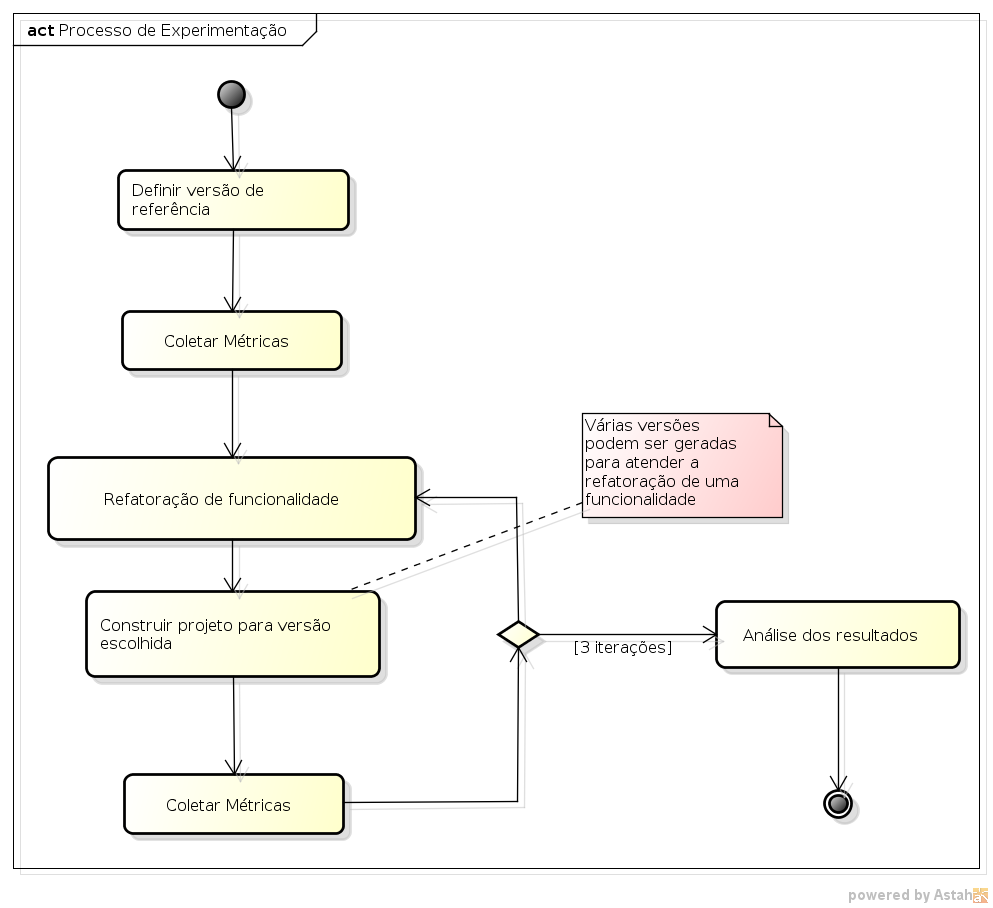
\includegraphics[scale=0.3]{img/processo_experimentacao.png}
	\end{center}
	
	\caption{\label{processo_experimentacao} Processo de Experimentação}
\end{figure}


\begin{itemize}
\item \textbf{Definir versão de referência} - Delimitar um marco do estado do
código no repositório.
\item \textbf{Refatoração de funcionalidade} - Esta atividade tem como
objetivo aplicar os padrões propostos em uma funcionalidade do aplicativo.
\item \textbf{Construir projeto} - Excutar o processo de construção do
projeto que inclui a compilação das classes para fazer a coleta das métricas.
\item \textbf{Coleta de Métricas} - Este passo tem como objetivo fazer a coleta
das métricas do código que se encontra no repositório a partir de uma revisão
para fazer a avaliação dos efeitos da refatoração na qualidade do código.
\item \textbf{Análise dos resultados} - Discussão dos impactos das alterações
executadas nas métricas.
\end{itemize}



\section{Trabalhos Relacionados}

O uso de um dispositivo móvel permite inovar ao usufrui-lo para atender
necessidades tanto para computação pessoal e corporativa. Conforme a variedade
de aplicativos surgem, o interesse em projeta-los com mais qualidade tambem
aumenta. Existem estudos sobre arquitetura de aplicativos Android como
demonstrado por \cite{BMVC}, onde é elaborado uma arquitetura baseada no
padrão de projeto MVC que é extendida para as camadas do sistema que estão
presentes em um serviço remoto para aproveitar as vantagens que a conectividade
desses aparelhos oferencem. Outro trabalho relacionado é
de \cite{corporateandroid} que desenvolvem um aplicativo dentro de um
contexto corporativo que é usado para consultar dados a partir de um banco de
dados central.

Não foi encontrado na literatura disponível, referências sobre a aplicação do
MVP para desenvolvimento de aplicativos android. Outros trabalhos mostram a
aplica- ção do padrão em outros contextos e plataformas  \cite{presenterfirst},
\cite{yangmvp}. Esses trabalhos enfatizam que o MVP melhora a
testabilidade, que é uma característica de qualidade de software.

A principal referência presente neste trabalho é \cite{cksuite} que
elaboram um conjunto de métricas para descrever de forma quantitativa a
qualidade de software orientado a objetos. \cite{cksuite} aplicam um
conjunto de seis métricas em dois projetos distintos desenvolvidos em Smalltak e
C++ analisando a relação dos resultados obtidos e os fatores que influenciaram
no desenvolvimento dos sistemas como por exemplo decisões arquiteturais e a
qualidade dos sistemas. Essas métricas serão usadas para avaliar a qualidade do
código resultante do processo de refatoração.

As métricas \cite{cksuite} tem se demonstradas como uma forma de avaliar a
qualidade de um sistema orientado a objetos. \cite{Dubey:2011} sumarizam
uma série de estudos que mostram o aumento da manutenabilidade do código ao
manter os valores das métricas baixos. Outras características de
qualidade de software são verificadas por meio de métricas de código
como demonstrado por \cite{Khalid:2010} que usa essas métricas para
avaliar a complexidade e a testabilidade de sistema orientados a objetos.
Segundo \cite{Briand:2000}, características como acoplamento, coesão e
herança estão relacionados com uma probabilidade maior de ocorrer falhas, e
avalia essa relação usando métricas para analisar a estrutura de projetos de
software. \cite{CK:98} relacionam os resultados dessas métricas com a
produtividade, esforço de retrabalho e projeto.

Na dissertação de \cite{turk} é feita uma análise dos impactos na
qualidade do código  ao aplicar cinco padrões de projetos em um software de comunicação
TCP/IP. Os resultados do trabalho citado mostram que a qualidade do software
aumenta ao aplicar padrões de projetos, sendo que o principal atributo de
qualidade aferido é a manutenabilidade. O método utilizado para a execução desta
pesquisa se baseia no trabalho citado. 

\section{Fundamentação Teórica}

\subsection{Princípios e Padrões de Projetos}


Desenvolver software orientado a objetos é um desafio. Criar uma representação
computacional de uma faceta da realidade em que seus constituintes trabalhem de
forma harmoniosa para atingir as necessidades que o software se propõe a
atender requer experiência, conhecimento do domínio do problema e um processo de
análise e projeto. Apesar de existirem várias abordagens para se conceber um
sistema orientado a objetos\cite{evans2004ddd},\cite{gomma11}, um sistema bem
construído apresenta características fundamentais como alta coesão e
baixo acoplamento.

A Coesão é uma característica de um componente de software que se refere ao grau
de relacionamento entres os membros desse componente. No contexto de uma classe,
é levado em consideração as relações entre os métodos e atributos. Classes com
coesão baixa demonstram grande complexidade pois os atributos e métodos que não
se relacionam indicam que a classe tem muitas responsablidades.

O acoplamento descreve as dependências entre componentes. Quanto maior a
quantidade dessas dependências entre classes, mais complexo ela se torna, pois
dificulta  alterações na classe. Além disso, o acoplamento aumenta o risco de
uma classe ser afetada devido à alterações em suas dependências.

Um padrão, dentro do contexto de estudo deste trabalho pode ser definido
como uma técnica efetiva cuja a sua aplicabilidade é aceita e difundida dentro
de uma área de conhecimento com a intenção de atingir um
objetivo\cite{MetskerWake06}. Ao seguir um padrão evita-se o retrabalho de
resolver um problema cuja a solução já existe.

Um padrão de projeto descreve uma solução para algum problema recorrente em um
sistema orientado a objeto \cite{gof}. Essa descrição envolve as motivações para
a utilização daquele padrão, a estrutura de classes e objetos participantes do
padrão e contextualização de sua aplicabilidade. Em desenvolvimento de software,
o catálogo mais difundido de padrões de projetos orientado a objetos é elaborado
por \cite{gof}, contendo um total de 23 padrões formalmente documentados
que acumulam experiências bem sucedidas em diversos sistemas. Esses padrões têm
a seguinte classificação:

\begin{itemize}
\item \textbf{Criacionais} - Padrões que definem como criar novas instâncias de
classes.
\item \textbf{Estruturais} -  Foca na estruturação das classes e objetos.\\
\item \textbf{Comportamentais} - Definem como as classes e objetos interagem
entre si e suas responsabilidades.
\end{itemize}
%argumentação
Analisando a forma como um padrão de projeto é concebido, com uma definição
dos papéis de cada elemento participante e como eles interagem entre si,
pode-se concluir que o uso dos padrões de projeto promove maior coesão, melhor
separação de interesses e baixo acoplamento no sistema. Todas essas
características contribuem para um software de melhor qualidade.


%Melhorar isso

%Linkar com as metricas, mostrar relação metricas e padroes

\subsection{Métricas de qualidade OO}
\label{sec:metrics}

%A qualidade de software . Segundo \cite{pressman}, qualidade de software 
%Qualidade

%Existem aspectos da qualidade de software que podem ser mensurados como
%Alguns aspectos da qualide de software são subjetivos, como por exemplo,
% a facilidade de uso ou manutenabilidade. É possível medir os 

%A classe é a unidade fundamental de um sistema oo

Com o advento de novas técnicas de desenvolvimento de software é necessário
obter informações do impacto dessas inovações nos resultados de um projeto. Com
esse objetivo \cite{cksuite} criaram um conjunto de métricas para
medir a qualidade de sistemas desenvolvidos usando o paradigma orientado a
objetos que não se limitasse a uma linguagem de programação, fácil de coletar e
com forte embasamento teórico na ontologia de Bunge que é um modelo usado pra
analisar algumas propriedades estáticas e dinâmicas de um sistema de
informação\cite{WandWeber}. As métricas são:

%Bunge’s ontology has
%considerable appeal for 00 researchers since it deals with the
%meaning and definition of representations of the world, which
%are precisely the goals of the object oriented approach [32]





\subsubsection{\textbf{Response sets for Class (RFC)}} Quantidade de métodos
que são executados quando um objeto recebe uma mensagem, incluindo os métodos de outras classes. É
levado em consideração somente os métodos que são chamados diretamente.

\begin{figure}[htb]
	\begin{center}
		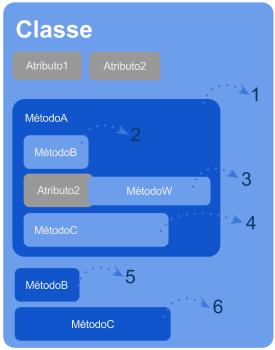
\includegraphics[scale=0.5]{img/pic_rfc.png}
	\end{center}
	\caption{\label{fig:pic_rfc}Exemplo de avaliação da métrica RFC}
\end{figure}


Na figura \ref{fig:pic_rfc}, a classe de exemplo tem um total de três métodos
definido nela. A implementação do método ``MetódoA'' chama o método ``MétodoB'',
o método ``MétodoW'' que é de outra classe referenciada pelo atributo
``Atributo2'' e o método ``MétodoC''. Assumindo que os métodos ``MétodoB'' e
``MétodoC'' não contém chamadas a nenhum outro método, o valor da métrica RFC
para a classe ilustrada é de seis métodos.

\subsubsection{\textbf{Wheighted Methods per Classe (WMC)}} Serve para expressar
o nível de complexidade de uma classe com base na soma da complexidade dos métodos que ela
possui. Isso afeta o esforço de manutenção da classe, além de impactar nas
classes filhas que herdarão esses métodos. Também é um indicativo de que a
classe tem métodos específicos dificultando o seu reuso. A unidade de
complexidade definida por \cite{cksuite} é o próprio método e não
considera outros fatores como número de linhas, número de parâmetros ou
quantidade de estruturas de decisão. A figura~\ref{fig:pic_wmc} ilustra como a
métrica WMC é avaliada em uma classe.

\begin{figure}[htb]
	\begin{center}
		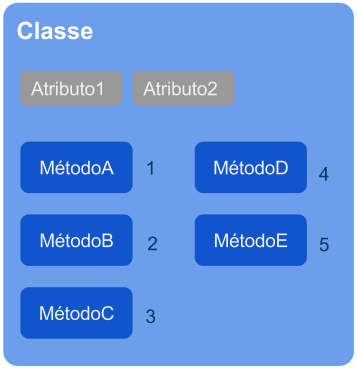
\includegraphics[scale=0.35]{img/pic_wmc.png}
	\end{center}
	\caption{\label{fig:pic_wmc}Exemplo de avaliação da métrica WMC}
	
\end{figure}

No exemplo da figura~\ref{fig:pic_wmc}, a classe reprensentada tem um total de
cinco métodos implementados. Seguindo estritamente o que \cite{cksuite}
definem para a métrica, o valor da métrica WMC para a classe é cinco métodos.


\subsubsection{\textbf{Coupling Bettwen Objects (CBO)}} Em um sistema orientado
a objetos, diversas classes são implementadas para exercer uma respoonsabilidade, as
instâncias dessa classes interagem entre si para atingir o objetivo do sistema.
Uma classe está acoplada a outra quando o método de um classe invoca o método de
uma variável de instância de outra classe que gera uma dependência entre essas
classes. Quanto mais dependências existirem, mais difícil é reutilizar esses
componentes em outras partes do sistema, além do aumento do risco de efeitos
colaterais que ocorrerem ao modificar uma classe altamente acoplada. O valor da
métrica CBO para uma classe é o número de outras classes que a classe analisada
depende.


\begin{figure}[htb]
	\begin{center}
		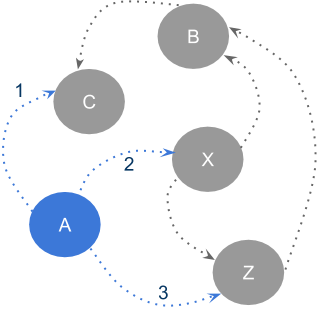
\includegraphics[scale=0.5]{img/pic_cbo.png}
	\end{center}
	\caption{\label{fig:pic_cbo}Exemplo de avaliação da métrica CBO}
	
\end{figure}

A figura \ref{fig:pic_cbo} ilustra um exemplo de acoplamento entre objetos. Um
classe chamada ``A'' depende das classes ``C'', ``X'' e ``Z''. O
valor de CBO para a classe ``A" é a somas de todas as suas
dependências, neste caso totalizando três dependências.


\subsubsection{\textbf{Depth Inheritance Tree (DIT)}}  Nível de uma classe na
hierarquia de herança. Reflete o número máximo de nós  dentro da árvore
de classes até a raiz, o que aumenta a complexidade conforme a quantidade de
elementos envolvidos se eleva, diminuindo a previsibilidade do comportamento da
classe com vários métodos e atributos sendo herdados, principalmente com o uso
de sobrecarga de métodos. No exemplo da figura \ref{fig:pic_dit} a classe
``ClasseZ'' tem um relacionamento de herança com a classe ``ClasseT'' que se
relaciona também por meio de herança com a classe ``Raiz''. A distância entre a
classe ``ClasseZ'' até a classe ``Raiz'' na hierarquia é de dois nós. Portanto o
valor da métrica DIT para a classe ``ClasseZ'' é dois.


\begin{figure}[htb]
	\begin{center}
		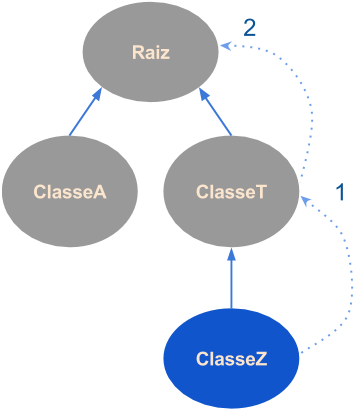
\includegraphics[scale=0.5]{img/pic_dit.png}
	\end{center}
	\caption{\label{fig:pic_dit}Exemplo de avaliação da métrica DIT}
	
\end{figure}


\subsubsection{\textbf{Lack of Cohesion in Methods (LCOM)}} Usado para avaliar a
coesão de uma classe por meio dos relacionamentos entre seus atributos e métodos.
O valor dessa métrica é fornecido por meio da quantidade de métodos que não tem
nenhum atributo em comum, menos a quantidade de métodos que tem atributos em
comum.

\begin{figure}[htb]
	\begin{center}
		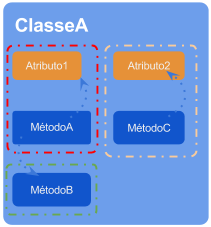
\includegraphics[scale=0.5]{img/pic_lcom_ex1.png}
	\end{center}
	\caption{\label{fig:pic_lcom_ex1}Exemplo  de avaliação da métrica LCOM}
	
\end{figure}

No exemplo da figura \ref{fig:pic_lcom_ex1} a classe ilustrada tem três métodos
implementados e cada método tem um conjunto de atributos que cada um utiliza.
O método ``MétodoA'' utiliza o atributo ``Atributo1'' formando o cunjunto Ma =
\{Atributo1\}, o método ``MétodoB'' não utiliza nenhum atributo formando um
conjunto vazio Mb = \{\}, e o método ``MetodoC'' referencia o atributo
``Atributo2'' formando o conjunto Mc = \{Atributo2\}. É necessário descobrir a
interseção de cada um desses grupos para saber quantos grupos tem atributos em
comum. A seguir é mostrado o resultado dessa avaliação:

\[
Ma \cap Mb = \{ \},
Ma \cap Mc = \{ \},
Mc \cap Mb = \{ \}
\]

Com esses resultados em mãos pode-se calcular o valor de lcom para a classe
exemplos. O total de conjuntos resultates vazios é três  e não foi identificado
nenhum conjunto com algum atributo que seja compartilhado entre os métodos.
Portanto o LCOM para para a classe ``ClasseA'' é, três conjuntos vazios, menos
zero conjuntos não vazios, que é igual a, LCOM três.

\subsubsection{\textbf{Number of Children (NOC)}} Número de subclasses imediatas
de uma classe analisada. Essa medida é um indicativo de mau uso de herança conforme seu
valor aumenta e mostra o impacto que uma classe pode ter no sistema requerendo maior
atenção e testes.

\begin{figure}[htb]
	\begin{center}
		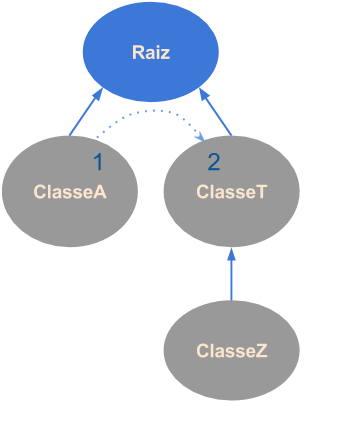
\includegraphics[scale=0.5]{img/pic_noc.png}
	\end{center}
	\caption{\label{fig:pic_noc}Exemplo de avaliação da métrica NOC}
	
\end{figure}

Na figura \ref{fig:pic_noc} a classe ``ClasseA'' e a classe ``ClasseT'' são as
únicas classes que tem uma relação de herança direta com a classe ``Raiz'',
portanto o valor da métrica NOC para a classe ``Raiz'' é  dois.


Todas essas métricas tem uma relação inerente com a coesão e acoplamento dos
objetos, sendo uma forma confiável para a análise da qualidade em sistemas
orientados a objetos. Os aplicativos desenvolvidos para a plataforma android são
escritos usando a linguagem de programação Java que emprega esse paradigma de
desenvolvimento, o que justifica o uso das métricas de \cite{cksuite} para
validação dos projetos orientados a objetos.

\subsection{Model View Controller}

O padrão \textit{Model View Controller} surgiu como uma solução genérica para
que usuários de um sistema de planejamento manipulem dados complexos
\cite{Reenskaug:1979}. Posteriormente, \cite{krasnerPope1988}
implementam um framework MVC para o ambiente gráfico da linguagem de programação
Smalltalk-80 como uma forma de promover a reusabilidade e plugabilidade dos
componentes de um sistema.

Segundo \cite{Reenskaug:1979} o principal objetivo do MVC
``\ldots é representar o modelo mental do usuário de um espaço de informações
relevantes e permitir que o usuário inspecione e altere estas
informações.''(tradução livre).
Esse modelo mental é como o usuário percebe o dominio do problema que está inserido no qual executará suas atividades sobre dados de seu interesse. Para que o usuário de um sistema de
informação possa interagir com a representação computacional  de seu modelo
mental três componentes são definidos:

Model - É o componente constituído de uma composição de classes que implementam
as regras de negócio referentes as funcionalidades que o programa provê,
representa o  conhecimento que o usuário tem e como manipulá-lo. Atende
mensagens da view requisitando seu estado e mensagens do controller para mudar
seu estado,

View - Representação específica de um model na interface com o usuário, é 
responsável por toda a manipulação visual, recuperando um estado do model e
exibindo os dados, podendo ser composta por sub-views e ser parte de views mais
complexas.

Controller - Interpreta as ações do usuário provenientes de um dispositivo de
entrada(Teclado, Mouse) alterando estado da view ou do model.


krasner and Pope \cite{krasnerPope1988} descrevem a estrutura do MVC onde a view
tem seu controller exclusivo mantendo uma dependência cíclica entre ambos. Tanto a View
quanto o Controller tem referências diretas para o model por meio de atributos
de classe, porém, o model não deve conhecer seus respectivos pares de
View-Controller para promover maior reuso de código e encapsulamento do model.
As alterações do estado do model são feitas na maioria das vezes pelo controller, e
o model é responsável por notificar todas as views que o representa para que
se atualizem refletindo o novo estado. No caso de um model ser usado por vários
pares de View-Controller as mensagens de notificação de um novo estado do model
podem ser parametrizadas assim cada view pode verificar se a alteração é de seu
interesse. 

Segundo \cite{Fowler:2002:PEA} ``\ldots esta separação da
apresentação e modelo é uma das mais fundamentais heurísticas de bom projeto
de software''(tradução livre).
O controller poderia ser o responsável por publicar as alterações no estado do
model devido sua relação direta com o mesmo, mas em casos onde o model é
alterado por outro componente que não é um dos controladores que os utilizam, é
necessário que o model conheça as views que devem ser notificados do novo
estado. Para que essas alterações de estado sejam propagadas a view e o
controller são registrados como dependentes de seu model. O padrão é descrito
levando em consideração as aplicações desenvolvidas em Smalltalk usando
características espefíficas dessa linguagem de programação que da suporte à
implementação dos três componentes como por exemplo o gerenciamento dos objetos
que são dependentes do model definido na classe Object que o model deve
extender. A Figura \ref{mvc} esclarece a interação entre os componentes.

\begin{figure}[htb]
	\begin{center}
		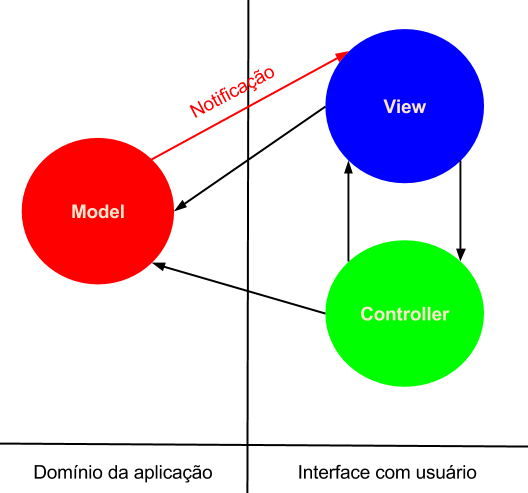
\includegraphics[scale=0.30]{img/mvc.png}
	\end{center}
	
	\caption{\label{mvc}Representação dos componentes do MVC}
\end{figure}


\subsection{Model View Presenter}

O MVP é um modelo de programação para implementação de interfaces com o usuário
desenvolvido como um framework para C++ e Java, criado por uma subsidiária da
IBM chamada Taligent,Inc. Este padrão é baseado no MVC e descreve vários
componentes que tem as responsabilidades de como gerenciar os dados da aplicação
e como o usuário interage com esses dados, tendo como objetivo promover o
encapsulamento do Model , reuso de lógica de negócio e o polimorfismo da View.
São Eles:

\begin{itemize}
\item \textbf{Model} - Tem as mesmas responsabilidades que o Model definido
pelo MVC.
\item \textbf{Selections} - Abstração para selecionar um subconjunto dos
dados existentes no model.
\item \textbf{Commands} - Representa as operações a serem executadas sobre
uma Selection do Model.
\item \textbf{View} - Responsável por exibir o model assim como no MVC.
\item \textbf{Interactor} - Mapeia os interações do usuário na view como
eventos do mouse.
\item \textbf{Presenter} - O papel do presenter é interpretar o eventos
iniciados pelo usuário executando a lógica de negócio correspondente implementada em um
  command para manipular o model \cite{Potel96mvp}.
\end{itemize}


Os conceitos do MVP são descritos em \cite{Potel96mvp} de forma genérica
permitindo interpretações para uma implementação efetiva.
\cite{twisttriad:2000} descrevem a implementação de um framework para
Dolphin Smalltalk\footnote{Implementação da Linguagem de programação Smalltalk - 
\url{http://www.object-arts.com}} adotando os conceitos do MVP onde salienta que
a maioria dos sistemas operacionais com ambiente gráfico fornece um conjunto de
componentes (Widgets) nos quais estão contidas as responsabilidades do
Controller, de acordo com a descrição do padrão MVC. A maior parte do
comportamento com o usuário é implementada no Presenter que está
diretamente associado à View.

Ainda acerca das responsabilidades do Presenter, \cite{fowler:ui} descreve
o que é chamado de Passive View, onde toda a lógica do comportamento da view é
implementado no presenter deixando a view enxuta com o intuito de isolar ao
máximo a API gráfica do resto da aplicação. Dessa forma o model não se comunica
com a view por meio do padrão Observer, sendo que a view séra atualizada
pelo presenter como pode ser observado na Figura~\ref{fig:mvp_passive_view}.

\begin{figure}[htb]
	\begin{center}
		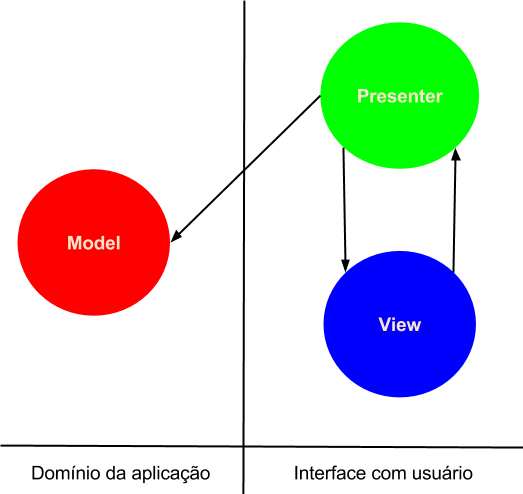
\includegraphics[scale=0.30]{img/passive_view.png}
	\end{center}
	\caption{\label{fig:mvp_passive_view} MVP - Passive View}
	
\end{figure}

Outra variação do MVP descrita por \cite{fowler:sp} é o Supevising
Controller. Nesta abordagem o Model utiliza algum mecanismo de notificação, por
exemplo o padrão Observer, para atualizar a View. Este comportamente é parecido
com o do padrão MVC como pode pode ser observado na
figura~\ref{fig:sup_controller}.

\begin{figure}[htb]
	\begin{center}
		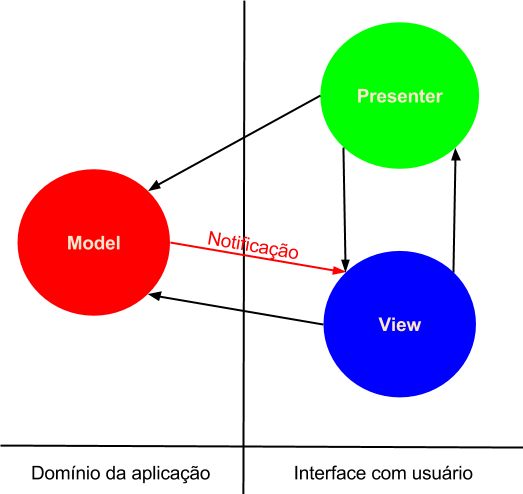
\includegraphics[scale=0.30]{img/supervising_controller.png}
	\end{center}
	
	\caption{\label{fig:sup_controller} MVP - Supervising Controller}
\end{figure}

MVP se adequa melhor as API's gráficas existentes e define de forma mais clara
os componentes necessários para desenvolver uma aplicação, sendo o ponto de maior
discussão reside em quais os limites das responsabilidades no que tange a
mediação do Model e a View por parte do Presenter.

\subsection{Framework Android}
 
O android é uma plataforma baseado no linux mantido pela Google para
ser embarcado em dispositivos podendo ser aplicado em carros, televisão, placas
controladoras mas seu destaque é a utilização em smartphones e
tablets, que é o foco deste trabalho. A plataforma é constituída por API's e
frameworks tendo em sua base o sistema operacional e seus drivers seguido da
máquina virtual que executa os aplicativos android e bibliotecas auxiliares e
aplicativos básicos. %como é demonstrado na figura \ref{android_stack}.

%\begin{figure}[htb]
%	\begin{center}
%		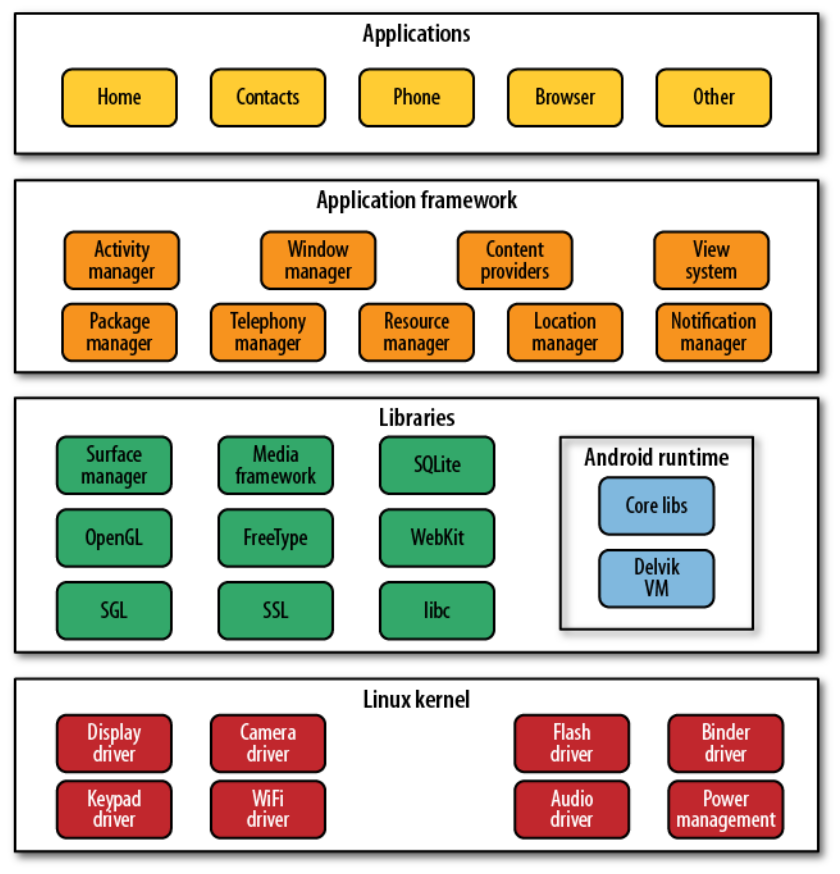
\includegraphics[scale=0.4]{img/android_stack.png}
%	\end{center}
%	\caption{\label{android_stack} Android Stack}
%\end{figure}

Para desenvolvimento é usada a API disponível no SDK que define
os blocos de construção de um aplicativo, a saber:

\begin{itemize}
  \item \textbf{Activity} - Representa uma atividade que o usuário executa no
  aplicativo em um determinado momento. É um agregador de componentes visuais e responde à
  interações do usuário.
  \item \textbf{Fragment} - Representa uma parte de interface com o usuário
  em uma Activity.
  \item \textbf{Service} -  Responsável por executar uma operação sem interface
  gráfica indicado para processamentos longos como por exemplo a execução de uma música
  ou download de de arquivos.
  \item \textbf{Broadcast Receiver} - Implementação do padrão
  publish/subscribe.
  \item \textbf{Content Provider} - Usado para expor dados de
  uma aplicativo para outros aplicativos. Os dados podem ser provenientes de qualquer forma de
  armazenamento como um arquivo ou banco de dados.
  \item \textbf{ApplicationContext} - Representa a aplicação em execução
  provendo acesso a recursos.
  \item \textbf{AsyncTask} - Usado para facilitar o uso de Threads evitando o
  uso da linha de execução principal do aplicativo que é respoonsável por tratar a
  interações com o usuário.
  
\end{itemize}


Com base nos componentes de framework e literatura revisada é possível fazer
uma análise dos mesmos e projetar uma camada de apresentação utilizando o padrão
MVP para ser usada como referência de implementação a ser aplicada.

\section{Execução da Pesquisa}


\subsection{Ferramentas Aplicadas}

O código será versionado no
Github\footnote{\url{https://github.com/diegofreitas/platform_packages_apps_contacts}}
onde será feito o gerenciamento das versões de cada iteração.
As ferramentas utilizadas para a refatoração serão a IDE Eclipse(Juno) com
plugin ADT v21 para facilitar a edição do código e ferramentas de construção
do projeto existentes no próprio repositório do android, tendo em vista que todo
o processo de compilação e empacotamento não visa ser usado em uma IDE.
Para realizar a coleta das métricas é necessário que a ferramenta analise código
java e contemple todas as métricas descritas na seção \ref{sec:metrics}. O
programa Chidamber and Kemerer Java
Metrics(CKJM)\footnote{\url{https://github.com/dspinellis/ckjm}} atende esses
critérios, além de ser um projeto de código aberto. O CKJM é uma aplicação java
sem interface gráfica, executado por linha de comando. Ele analisa o código java
compilado, conhecido como byte codes contido em arquivos com extensão .class. Um
exemplo de uso do CKJM é mostrado a seguir:

\begin{figure}[htb]
	\begin{center}
		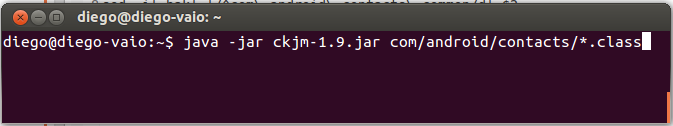
\includegraphics[scale=0.30]{img/ckjm_run.png}
	\end{center}
	\caption{\label{fig:ckjm_run} Exemplo de execução do CKJM} 
	
\end{figure}

Os resultados são escritos na saída padrão do sistema, neste caso, no terminal
de execução, mostrando uma lista com os nomes completos das classes
analisadas, seguidas dos respectivos valores das métricas na seguinte
ordem: WMC, DIT, NOC, CBO, RFC, LCOM, Ce, and NPM sendo que as métricas Ce e
NPM são desconsideradas para esta pesquisa. a figura~\ref{fig:ckjm_result}
ilustra o resultado de uma coleta.

\begin{figure}[htb]
	\begin{center}
		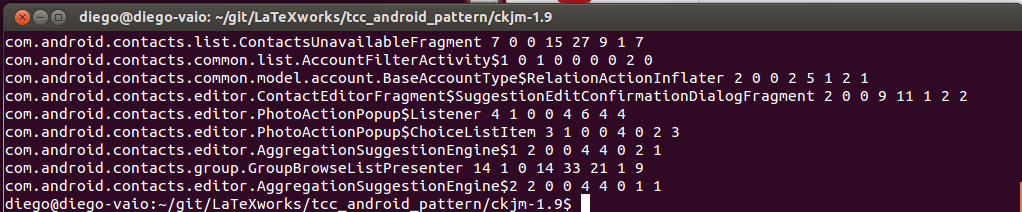
\includegraphics[scale=0.25]{img/ckjm_result.png}
	\end{center}
	\caption{\label{fig:ckjm_result} Exemplo de resultado da análise do CKJM} 
	
\end{figure}


\subsection{Análise do objeto de estudo}

O aplicativo a ser refatorado tem funcionalidades para gerenciamento de
contatos e é composto 153 classes organizadas em 13 pacotes. O padrão
de projeto MVP será aplicado em uma parte do aplicativo. Será refatorado o
pacote referente ao gerenciamento de grupos de contatos presente no pacote
\textbf{com.android.contacts.group}. A figura \ref{fig:pacotes_contacts}
mostra os pacotes que compõem o aplicativo. O pacote a ser refatorado está
destacado em azul.

\begin{figure*}[htb]
	\begin{center}
		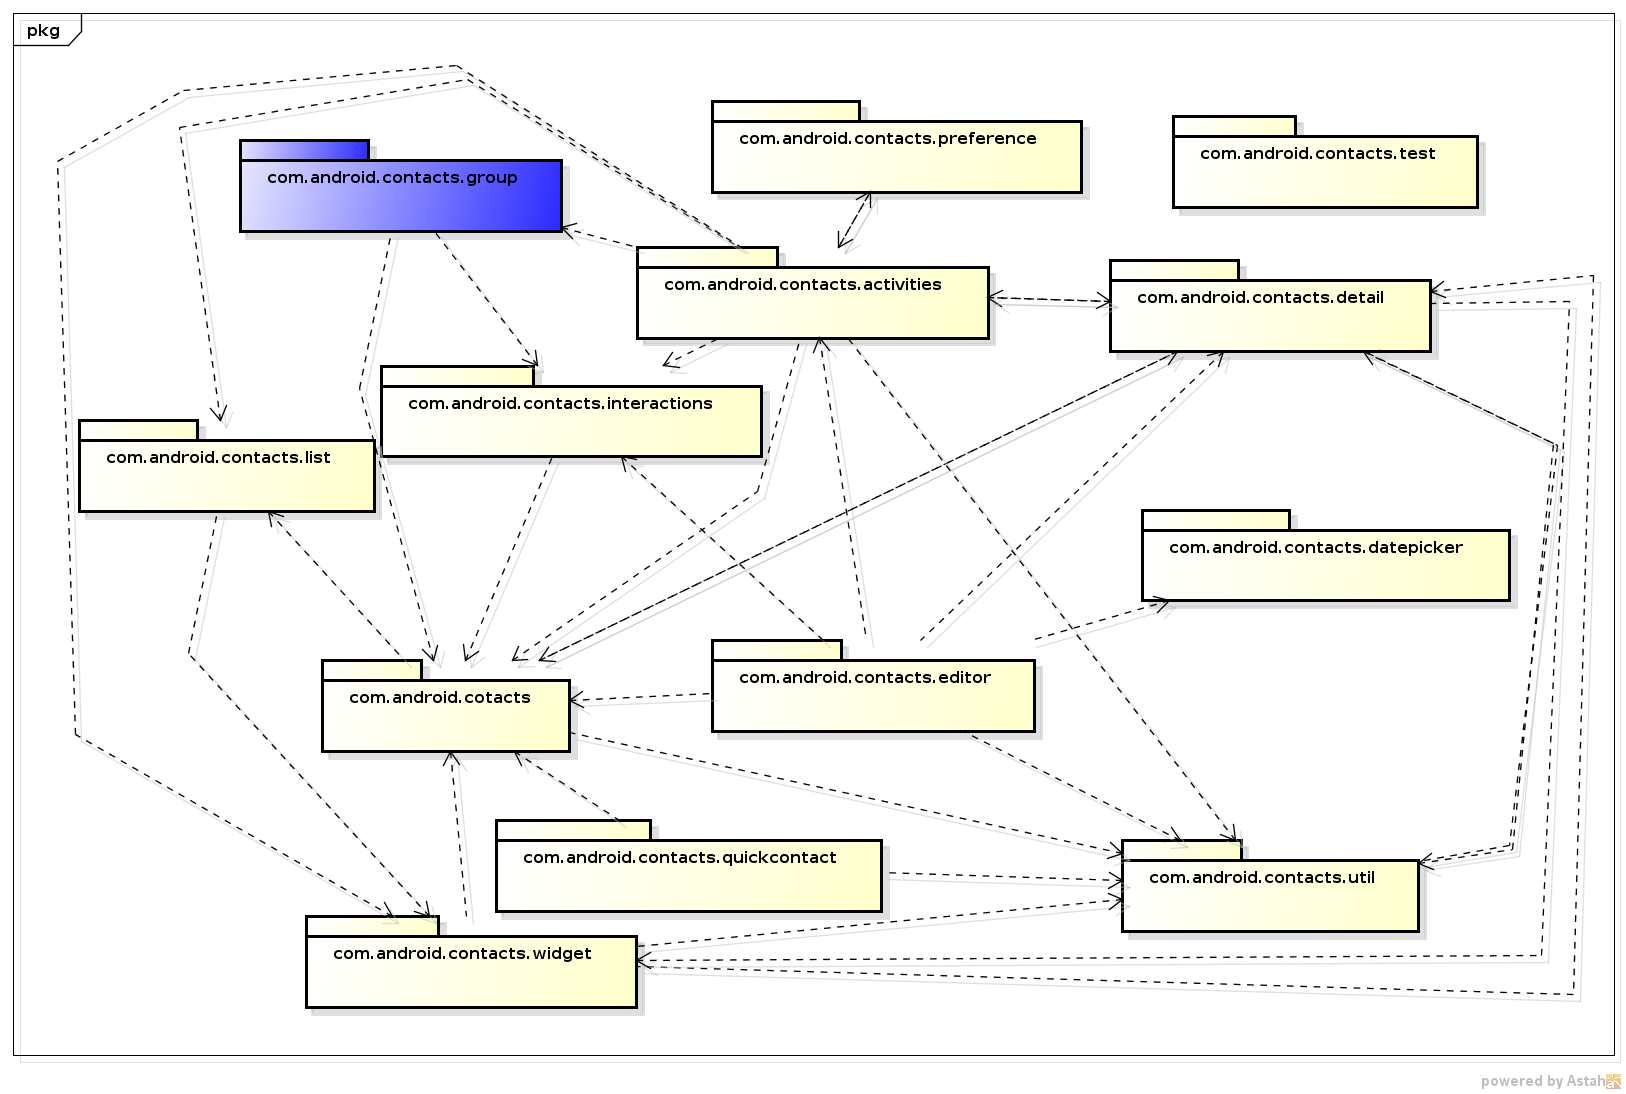
\includegraphics[height=8cm,width=\textwidth]{img/pacotes_contacts.png}
	\end{center}
	\caption{\label{fig:pacotes_contacts} Diagrama de pacotes do aplicativo de contatos}	
\end{figure*}

A cada iteração será selecionada uma tela do aplicativo para a aplicação do
padrão MVP. Cada tela é implementada por uma classe e suas interfaces
são ilustradas nas figuras \ref{fig:contacts_groups},
\ref{fig:contacts_groups_view} e \ref{fig:groups_edit}. 

\begin{figure}[htb]
	\centering
	\begin{minipage}[b]{0.45\linewidth}
		\begin{center}
			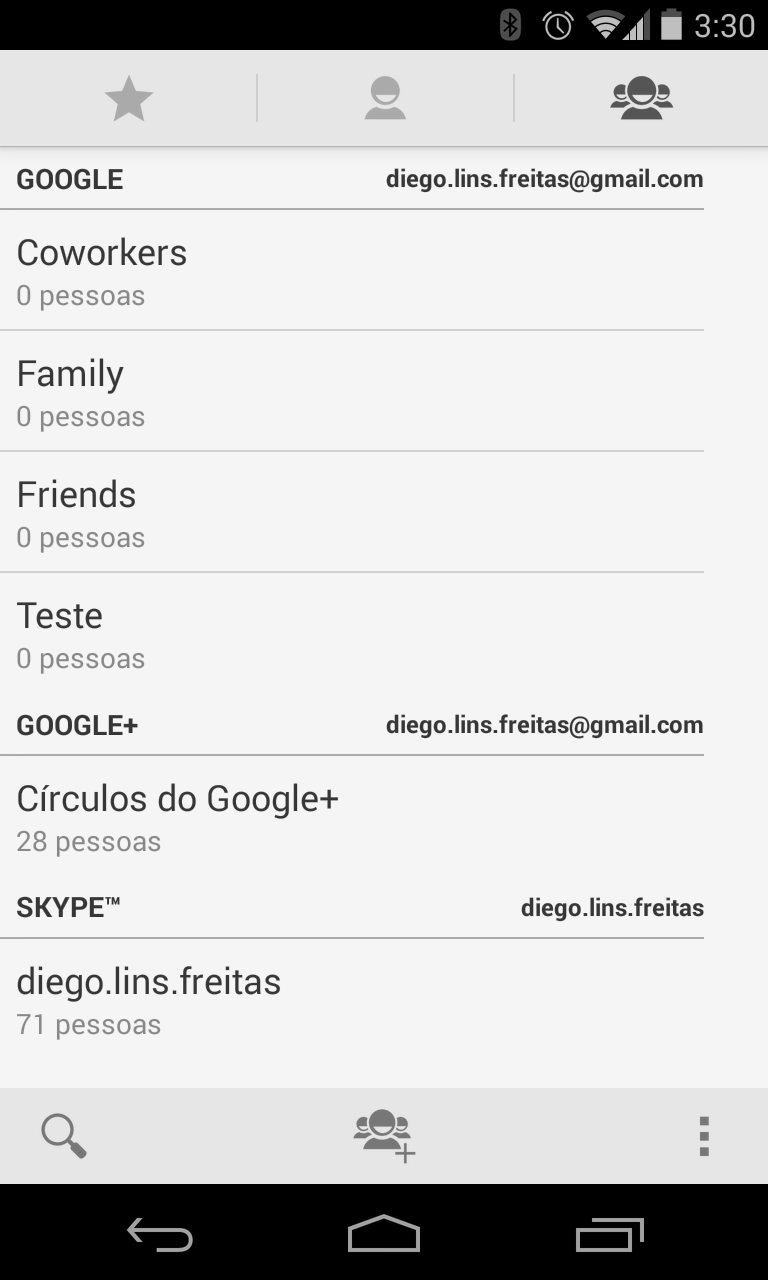
\includegraphics[scale=0.15]{img/contacts_groups.png}
		\end{center}
		\caption{\label{fig:contacts_groups} Tela de lista de grupos} 
		
	\end{minipage}
\quad
	\begin{minipage}[b]{0.45\linewidth}
		\begin{center}
			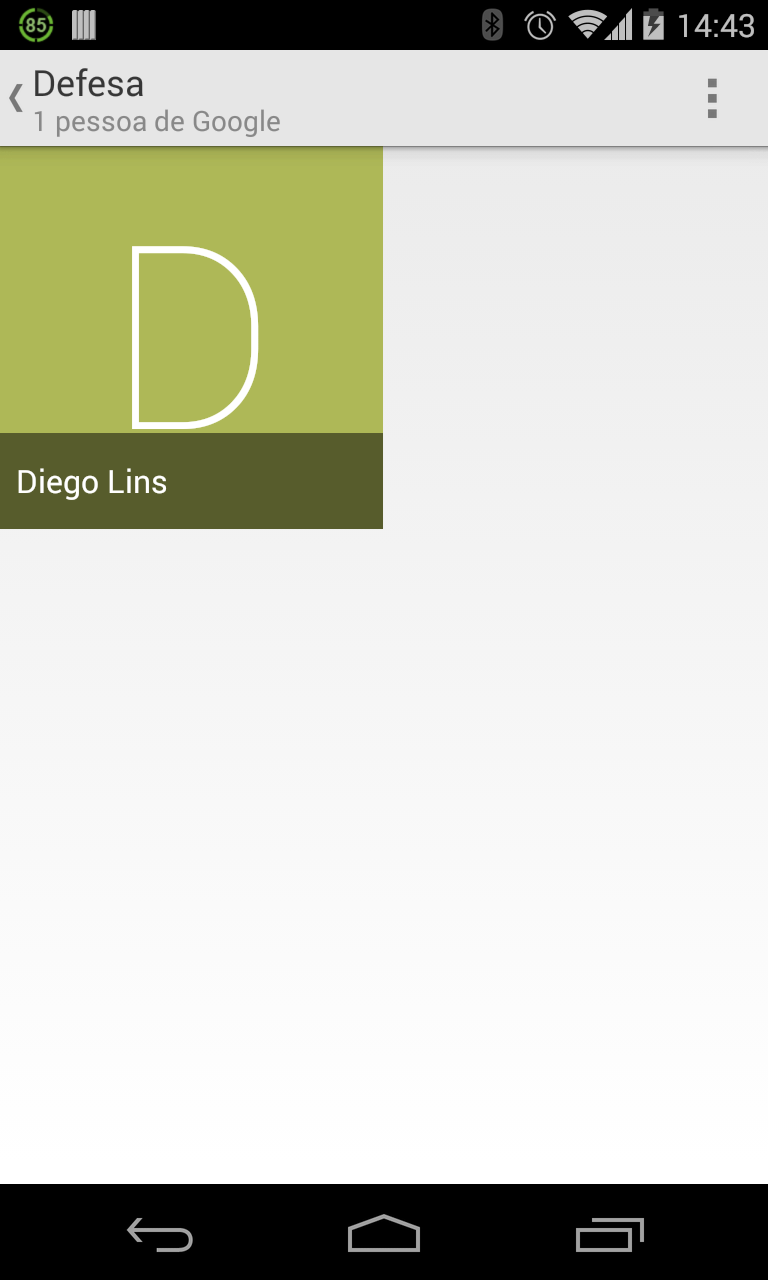
\includegraphics[scale=0.15]{img/contacts_group_view.png}
		\end{center}
		\caption{\label{fig:contacts_groups_view} Tela de visualização de um grupo}
		 
	\end{minipage}
\quad
	\begin{minipage}[b]{0.45\linewidth}
		\begin{center} 
			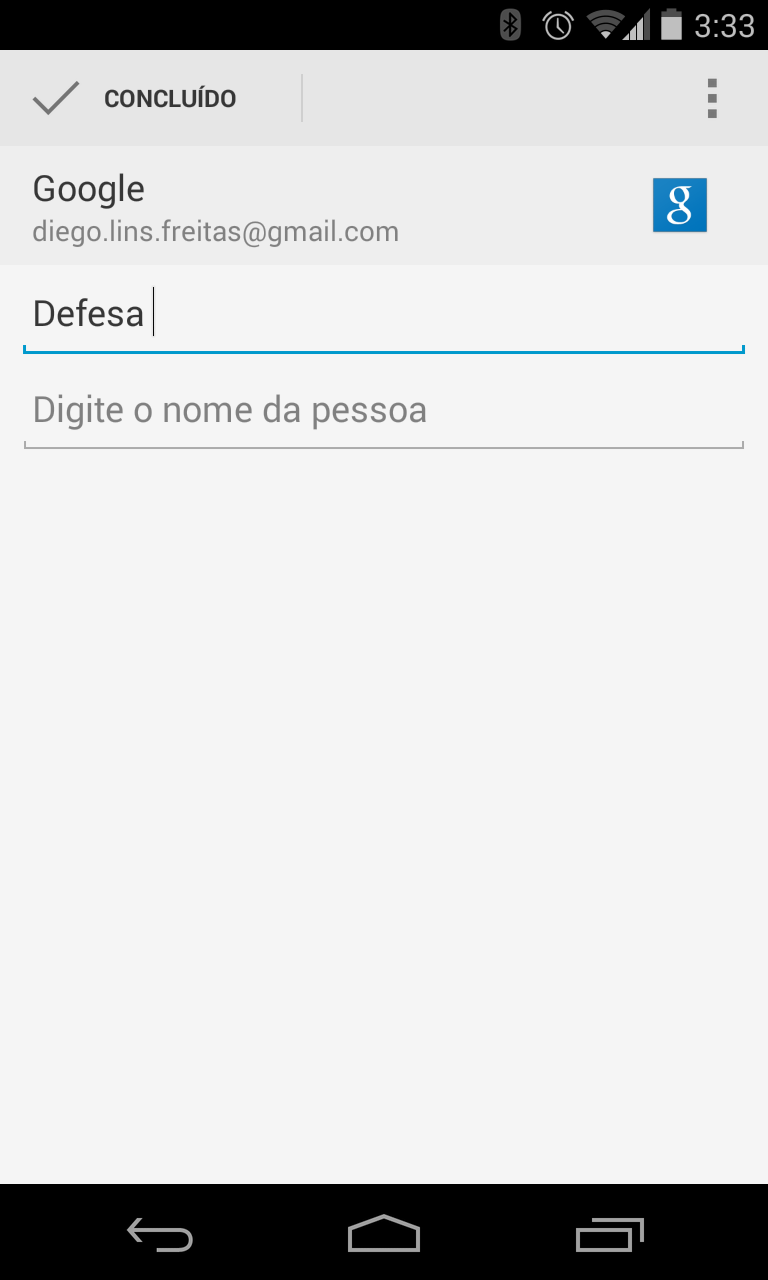
\includegraphics[scale=0.15]{img/contacts_edit.png}
		\end{center}
		\caption{\label{fig:groups_edit} Tela de edição e criação de grupos}
		 
	\end{minipage}
\end{figure}


As classes a serem refatoradas são:

\begin{itemize}
\item \textbf{GroupDetailFragment.java} -  Exibe os dados de um grupo de
contatos.
\item \textbf{GroupBrowseListFragment.java} - Fornece uma lista de grupos.
\item \textbf{GroupEditorFragment.java} - Disponibiliza um formulário para
edição dos dados de um grupo.
\end{itemize}

Essas classes estão presentes no pacote \textbf{com.android.contacts.group} como
mostra a figura \ref{fig:classes_group_baseline}.

\begin{figure}[htb]
	\begin{center}
		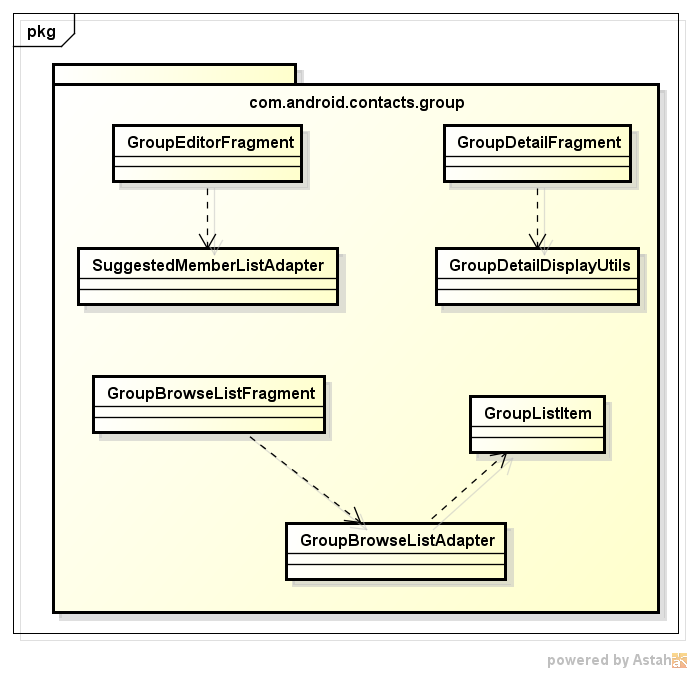
\includegraphics[scale=0.4]{img/classes_group_baseline.png}
	\end{center}
	\caption{\label{fig:classes_group_baseline} Diagrama de pacotes de grupos}   
\end{figure}

Estas interfaces com o usuário são usadas dentro de Activities que controlam uma
parte do fluxo de interação e se comportam de forma diferente conforme o tipo de dispositivo
móvel utilizado (tablet ou smartphone). Devido a essa complexidade, não será
feita nenhuma alteração na interface pública dos componentes refatorados, evitando efeitos colaterais em
outras partes do aplicativo. Os componentes elencados contêm código não somente
relacionado com a lógica de apresentação como também interagem diretamente com classes destinadas ao acesso
de dados e serviços existentes nas dependências do projeto, por exemplo,
gerenciamento de contas do usuário.  Cada iteração consistirá na refatoração de
cada um dos componentes descritos. O marco de referência de dados das métricas presentes na tabela \ref{tab:dados_baseline} será feita a partir da
versão \verb|4.4.2_r1| do aplicativo.

\begin{table}[!h]
	\centering
	    \caption{\label{tab:dados_baseline} Métricas CK da versão de referência}
	
    \begin{tabular}{ | l | l | }
    \hline
    Métrica &	Média \\ \hline
    WMC  	&	8.5161290323   	\\ \hline
    DIT	 	&	0.7741935484	\\ \hline
	NOC  	& 	0				\\ \hline
	CBO	  	& 	10.1612903226	\\ \hline
	RFC	 	& 	23.7419354839	\\ \hline
	LCOM 	& 	57.4838709677	\\ \hline
    \end{tabular}
    
\end{table}


Os dados de referência apresentados na tabela \ref{tab:dados_baseline} foram
coletados usando a ferramenta CKJM. Os dados são referentes ao pacote de grupos.
Foram coletados os valores de cada métricas para cada uma das classes presentes
no pacote de grupos e para cada métrica foi calculado a média. A cada
refatoração será executado o mesmo procedimento de coleta descrito para fazer
uma análise na variação das médias de cada métrica.


\subsection{Arquitetura Proposta}

Será aplicado nos experimentos a variação do padrão MVP chamada Passive View,
pois dessa forma, o Model não precisa publicar alterações de seu estado para a
view, Logo, evita-se alterações no código referente às classes que fazem
parte da camada de Model do aplicativo de contatos. A organização do código
fonte no repositório dificulta a implementação, isto porque esses componentes estão
localizados fora do projeto afetado e são compartilhados.

As classes que extendem Fragment terão a responsabilidade da View, pois é neste
componente que a interface com o usuário é construída. A classe Activity fornece
vários métodos para recuperação de recursos de imagens, textos, inicialização de
serviços, entre outros. Isso ocorre porque a classe Activity é uma subclasse de Context, herdando diversos métodos não relacionados ao gerenciamento da interface.

Segundo \cite{Reenskaug:1979} ``\ldots Os papéis da View e do
Controller podem ser exercidos pelo mesmo objeto quando eles estão muito
acoplados. Exemplo: Um Menu.''(tradução livre). Porém, isso requer um boa
análise do problema em questão para decidir o nível de granularidade que esses componentes podem ter.
Portanto, é recomendável manter sempre essa separação para manter uma boa coesão
nas classes. O Presenter será uma classe auxiliar à View e pode ser implementada
como uma classe java simples. 



\subsection{Resultados dos Experimentos}

Esta seção tem como objetivo mostrar os resultados obtidos com o processo de
refatoração aplicando o parão MVP. Cada métrica é apresentada com seus dados
para cada iteração mostrando os efeitos desses valores na qualidade.

\subsubsection{WMC}

%qual o cenario ideal para metrica;
A métrica WMC é usada para medir o tempo e esforço necessário para desenvolver e
manter uma classe. Levando em consideração o método como uma unidade de
complexidade, quanto menos métodos um classe tiver menos complexa ela será,
portanto, é recomendado que esta métrica tenha valores baixos.
Entretanto, uma classe terá a quantidade de métodos necessária para exercer seu
papel no sistema. É inviável desenvolver um sistema cujas todas as classes
tenham um único método com a implementação de todas as funcões de uma
classe. Portanto, não existe um valor ideal para a métrica WMC. Essa métrica
deve ser analisada levando em consideração o contexto da classe de interesse além da
complexidade expressa pela quantidade de métodos. 

A possibilidade de reuso de uma classe reduz, pois a grande quantidade de
métodos indica que ela tem funções muito específicas\cite{cksuite}. Neste caso o
WMC é um indicador de que é necessário fazer um refatoração para extrair funções comuns a outras partes do
aplicativo, além do pacote de Groups, como por exemplo funções para exibição de
dados em uma lista, validação de dados em componentes de texto, entre outros. O
escopo de atuação do padrão MVP é mais amplo, abrangendo o caso de uso realizado pela
interface refatorada. Logo, o MVP não tem impacto na reusabilidade.

Os efeitos colaterais em uma classe filha é maior quando é feito alguma
alteração na classe pai que tenha o número de métodos muito alto\cite{cksuite}.
Isso dificulta a manutenabilidade e o esforço de testes. Porém, As classes
refatoradas tem uma função muito específica dentro da aplicação e não são
extendidas por outras classes. O MVP está relacionado com a separação de
responsabilidades e sua aplicação não interferiu na hierarquia de classes que
foram refatoradas.
A tabela \ref{tab:wmc} e a figura \ref{fig:wmc} mostram os valores dessa
métrica no projeto.


\begin{table}[!h]
	\centering
	\caption{\label{tab:wmc}Dados métrica WMC}
    \begin{tabular}{ | l | l | }
    \hline
    Iteração & Média 			\\ \hline
    Baseline & 8.5161290323   	\\ \hline
    Iteração 1 & 8.875			\\ \hline
	Iteração 2 & 9				\\ \hline
	Iteração 3 & 8.9393939394	\\ \hline
    \end{tabular}
    

\end{table}


\begin{figure}[!htb]
	
	\begin{center}
		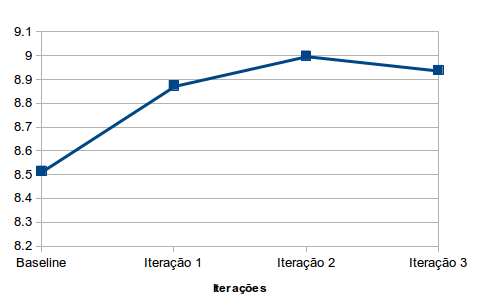
\includegraphics[scale=0.75]{img/wmc.png}
	\end{center}
	\caption{\label{fig:wmc} Gráfico da métrica WMC}   
	
\end{figure}


%3o) justificar o q causou tal comportamento.

De acordo com o que foi exposto, o MVP não deveria afetar a métrica WMC. Porém,
houve um aumento nos valores dessa métrica . Isso é consequência da divisão de
responsabilidades entre a View e o Presenter. Antes da refatoração, os métodos
das classes de View implementavam o acesso a dados, controle dos componentes
visuais e regras específicas das operações executadas na tela, como por exemplo,
a atualização de um componente visual quando nenhum dado está disponível para
exibição. Os métodos da classe de View, afetados pela refatoração, foram
dividídos em no mínimo dois métodos. Sendo que, o método que permanece na View
manipula os componentes visuais, enquanto o novo método criado no Presenter faz
o acesso à camada de Model e implementa as regras de negócio da operação em
resposta à interação do usuário na View. Como consequência a quantidade de
métodos aumenta, porém, os métodos tornam-se mais simples pois implementam
funcões específicas. 

Levando isso em consideração, apesar dos valores de WMC
terem aumentado, a complexidade diminuiu, pois os métodos estão mais concisos.
No contexto dessa refatoração, a métrica WMC não pode ser considerada um
indicador determinante para a avaliação da qualidade do objeto de estudo.


\subsubsection{NOC}

Altos valores para a métrica NOC são indicativos de que existe maior reuso de
código. Assim como DIT, a métrica NOC é um indicador da influência da classe
no comportamento das classes filhas o que aumenta o esforço de testes. Quando os
valores desta métrica estão aberrantes em relação às outras classes, há grande
chance de que a abstração está sendo usada de forma incorreta. Dado esses cenários, está é um métrica cujos
seus valores devem ser analisados caso a caso.

Durante o processo de refatoração não foi aplicada herança em nenhuma das
classes afetadas, portanto, essa métrica permaneceu intacta durante as iterações
como pode ser observado na tabela \ref{tab:noc}. %e figura~\ref{fig:noc}

\begin{table}[!h]
	\centering
	    \caption{\label{tab:noc} Dados métrica NOC}
    \begin{tabular}{ | l | l | }
    \hline
    Iteração & Média 			\\ \hline
    Baseline & 0  	\\ \hline
    Iteração 1 & 0			\\ \hline
	Iteração 2 & 0				\\ \hline
	Iteração 3 & 0	\\ \hline
    \end{tabular}
    
\end{table}

%\begin{figure}[h]
%	\centering
%	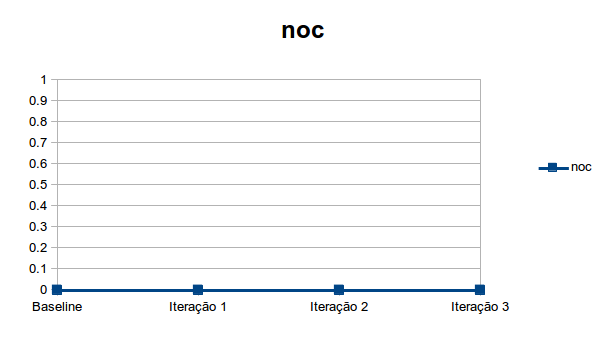
\includegraphics{img/noc.png}
%	\caption{Valores de NOC/Fonte: Próprio autor}
%	\label{fig:noc}
%\end{figure}


\subsubsection{DIT}

A métrica DIT está relacionada complexidade e reusabilidade. Quanto mais
abaixo na hierarquia de herança a classe estiver, menos previsível será seu
comportamento devido a quantidade de métodos que serão herdados das classes
acima nessa hierarquia. Entretanto, a métrica também indica um potencial reuso
de código por meio da herança de métodos, isso torna os parâmetros de avaliação
da métrica dependentes do contexto a ser analisado. O aumento demonstrado na DIT
se deve ao fato que o CKJM considera a implementação de interface como herança.
A interface define somente o contrato que a classe deve implementar. Sendo uma
interface, não há nenhuma implementação que possa interferir no comportamento
da classe, portanto essa alteração na métrica DIT não deve ser considerada. O
aumento no valor da métrica é mostrado na tabela~\ref{tab:dit} e
figura~\ref{fig:dit}

\begin{table}[!h]
	\centering
	    \caption{\label{tab:dit} Dados métrica DIT}
    \begin{tabular}{ | l | l | }
    \hline
    Iteração & Média 			\\ \hline
    Baseline & 0.7741935484  	\\ \hline
    Iteração 1 & 0.78125		\\ \hline
	Iteração 2 & 0.78125			\\ \hline
	Iteração 3 & 0.7878787879	\\ \hline
    \end{tabular}
    
\end{table}

\begin{figure}[!htb]
	\begin{center}
		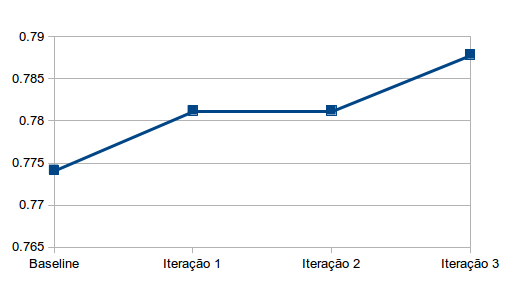
\includegraphics[scale=0.7]{img/dit.png}
	\end{center}
	
	\caption{\label{fig:dit} Gráfico da métrica DIT}   
\end{figure}

\subsubsection{CBO}

Valores baixos de CBO são indicativos de boa modularidade e encapsulamento que
se reflete na independência da classe, o que a torna mais fácil de reutilizar,
manter e testar.
Na primeira iteração foi aplicado o padrão em um componente mais simples e foi
possível remover qualquer dependência que não fosse relacionada a interface,
diminuinido significativamente o valor da métrica. Nas iterações seguintes foram
refatoradas interfaces mais complexas onde é mais difícil desacoplar as
dependências. Algumas depedências não relacionadas a camada de apresentação
permaneceram na View, dessa forma, tanto a View como o Presenter tem referências
para essas dependências aumentando o valor da métrica. Além disso, existe o
acréscimo de duas dependências entre a View e o Presenter. A variação da métrica
é exposta na tabela \ref{tab:cbo} e na figura~\ref{fig:cbo}

\begin{table}[!h]
	\centering
	    \caption{\label{tab:cbo} Dados métrica CBO}
	
    \begin{tabular}{ | l | l | }
    \hline
    Iteração & Média 			\\ \hline
    Baseline & 10.1612903226   	\\ \hline
    Iteração 1 & 10.03125		\\ \hline
	Iteração 2 & 10.09375		\\ \hline
	Iteração 3 & 10.1515151515	\\ \hline
    \end{tabular}
    
\end{table}

\begin{figure}[!htb]
	\begin{center}
		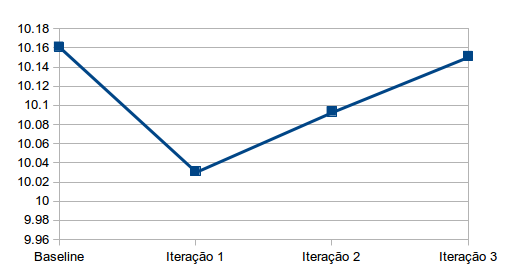
\includegraphics[scale=0.7]{img/cbo.png}
	\end{center}
	\caption{\label{fig:cbo} Gráfico da métrica CBO}   
	
\end{figure}


\subsubsection{RFC}

Altos valores para a métrica RFC indica que uma quantidade grande de métodos são
chamados a partir de uma classe tornando-a mais complexa de testar e fazer
manutenção. Logo, esta métrica deve deve diminuir para expressar maior
qualidade no código. A métrica RFC tende a aumentar a cada iteração, o que
sugere um aumento da complexidade do código conforme é apresentado na tabela \ref{tab:rfc} e Figura
\ref{fig:rfc}.

\begin{table}[!h]
	\centering
	    \caption{\label{tab:rfc} Dados métrica RFC}
    \begin{tabular}{ | l | l | }
    \hline
    Iteração & Média 			\\ \hline
    Baseline & 23.7419354839   	\\ \hline
    Iteração 1 & 24.21875		\\ \hline
	Iteração 2 & 24.71875		\\ \hline
	Iteração 3 & 24.9090909091	\\ \hline
    \end{tabular}
    
\end{table}

\begin{figure}[htb]
	\begin{center}
		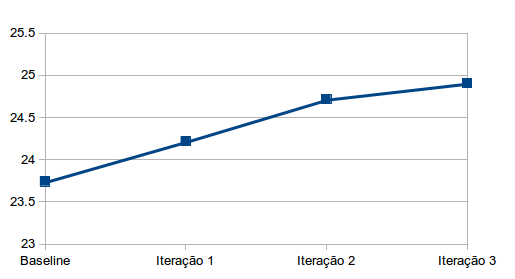
\includegraphics[scale=0.7]{img/rfc.png}
	\end{center}
	\caption{\label{fig:rfc} Gráfico da métrica RFC}   
	
\end{figure}


A justificativa para o aumento da métrica WMC também se aplica neste caso.
Após cada iteração de refatoração, as Views passaram a delegar
responsabilidades para o Presenter por meio de chamada de métodos, além disso, o Presenter interage com a
View da mesma forma para atualizá-la. Portanto, a quantidade de chamada de
métodos aumentaram e isso se refletiu na métrica RFC.

\subsubsection{LCOM}

Segundo \cite{cksuite} ``Um valor alto de LCOM indica uma disparidade na
funcionalidade provida pela classe.". Analisando a relação entre os métodos da
classe e seus atributos é possível dizer se a classe tem muitas
responsabilidades e é necessário dividi-la em duas ou mais classes. Esta métrica
ajuda a identificar má qualidade na estrutura do código quando os valores são
altos, apontando aumento da complexidade e pouco encapsulamento. A tabela
\ref{tab:lcom} e a figura \ref{fig:lcom} mostram uma queda siginificativa na
métrica LCOM. Isto indica que a coesão do código melhorou após cada iteração.

\begin{table}[!h]
	\centering
	    \caption{\label{tab:lcom} Dados métrica LCOM}
    \begin{tabular}{ | l | l | }
    \hline
    Iteração & Média 			\\ \hline
    Baseline & 57.4838709677   	\\ \hline
    Iteração 1 & 56.875			\\ \hline
	Iteração 2 & 53.1875		\\ \hline
	Iteração 3 & 48.4242424242	\\ \hline
    \end{tabular}
    
\end{table}

\begin{figure}[!htb]
	\begin{center}
		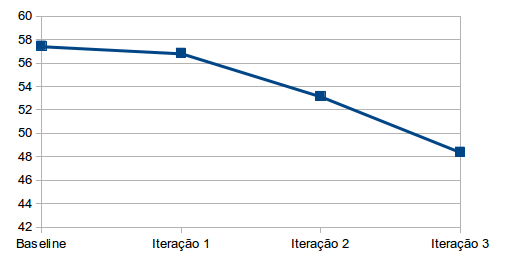
\includegraphics[scale=0.5]{img/lcom.png}
	\end{center}
	\caption{\label{fig:lcom} Gráfico da métrica LCOM}   
	
\end{figure}



\subsection{Discussão dos Resultados} 




%CBO
As classes destinadas à implementação da interface no framework android fornecem
acesso a recursos que servem para implementação de responsabilidades não
relacionadas com a interface. Essa característica do framework android leva à
implementação da camada de View com diversas responsabilidades que não são
inerentes à interação com o usuário. Isso dificultou a refatoração, pois as
classes que exercem o papel de Presenter necessitam interagir com as classes de
View para acessar esses recursos, além de atualizar o estado da View. O uso do
padrão de injeção de
dependência\footnote{Padrão
de projeto onde um objeto recebe as referências para as suas dependências sem
conhecer os processo de contrução das mesmas.
\url{http://en.wikipedia.org/wiki/Dependency_injection}}
pode ser aplicado para acessar esses recursos e serviços sem a necessidade de
interação com a classe de View.

Houve diminuição na métrica CBO nas classes alteradas pois diversas
responsabilidades que utilizam essas dependências foram movidas para a classe de
Presenter. Analisando de forma geral, essas dependências permanecem no pacote
além de ser criado mais um acoplamento entre a View e a nova classe Presenter.
A figura \ref{fig:classes_iteracao3} mostra a disposição das classes após a
refatoração.

\begin{figure}[htb]
	\begin{center}
		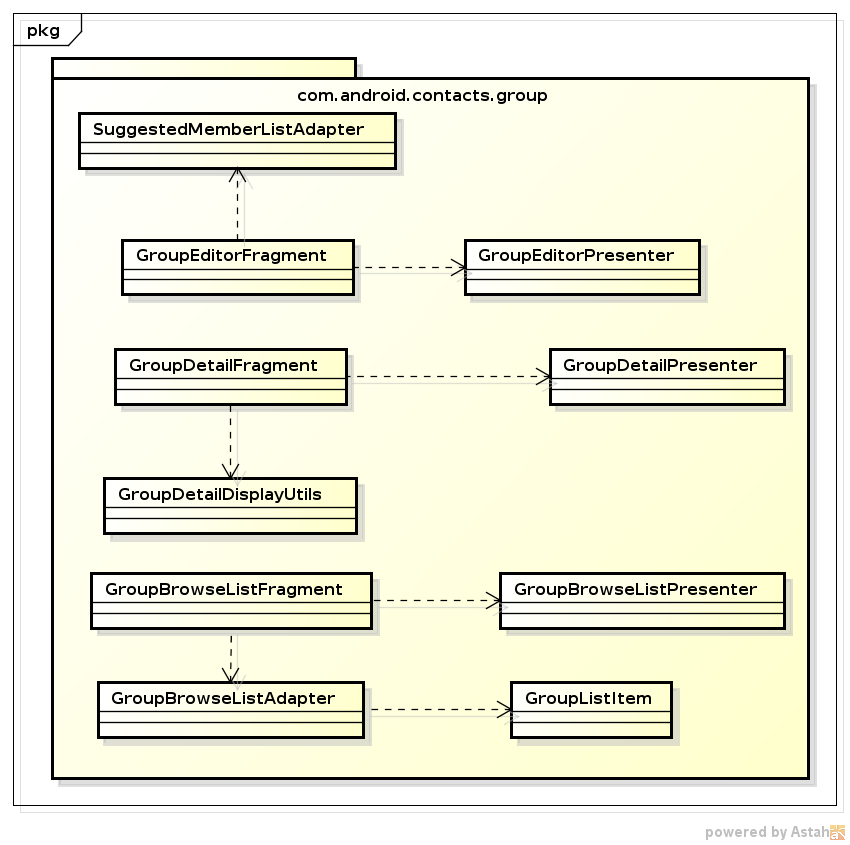
\includegraphics[scale=0.3]{img/classes_iteracao3}
	\end{center}
	\caption{\label{fig:classes_iteracao3} Pacote após refatoração}
	
\end{figure}

%WMC/RFC OK
Ao usar o padrão MVP, a quantidade de linhas de métodos diminui pois cada um
dos componentes implementaram uma parte do caso de uso, aumentando o números de
métodos que se reflete na métrica WMC. Na implementação original onde um método
que era implementado na classe View, tinha a  responsabilidade de tratar os
eventos do usuário, acessar os componetes visuais e recuperar os dados, validar
esses dados, acessar o Model para persistir o dados e atualizar a tela como o
novo estado. Tudo isso resulta em métodos com muitas linhas de código com várias
estruturas de controle e iteração, isso aumenta a complexidade da classe.

Ao dividir as responsabilidades entre os componentes definidos no padrão, um
método complexo que era implementado na View quebrado em pelo menos três métodos
menores, para que a View possa receber as interações com o usuário e dados de
entrada para então delegar o precessamento ao Presenter que vai interagir com as
classes que exercem o papel de Model, e para finalizar, o Presenter chama algum
método da View que irá atualizar os componetes visuais com o novo estado dos
dados.

Tendo em vista que o método foi usado como unidade para calcular o WMC, essa
métrica aumentou ao aplicar o padrão MVP, pois mais métodos foram criados. A
métrica WMC mostra a complexidade de uma classe, mas apesar do aumento nos
valores, a complexidade diminuiu, ao ser usado a implementação com métodos mais
simples.
% colocar imagem de código antes e depois.
A divisão de responsabilidades também afetou negativamente a métrica RFC, pois
com o aumento da quantidade de métodos, a troca de mensagens entre componentes
e com a própria classe aumentaram.  


A métrica WMC está relacionada com as métricas DIT e NOC. Como houve pouca
variação no DIT e nenhuma variação no NOC, o aumento da WMC não tem impacto
relevante.

Os experimentos demonstraram que a aplicação do padrão MVP promoveu de forma
significativa maior coesão no aplicativo. Isso é demonstrado nos resultados da
métrica LCOM que foi a mais afetada pelo uso do padrão MVP no projeto como pode
ser observado na figura \ref{fig:allmetrics}.

\begin{figure}[htb]
	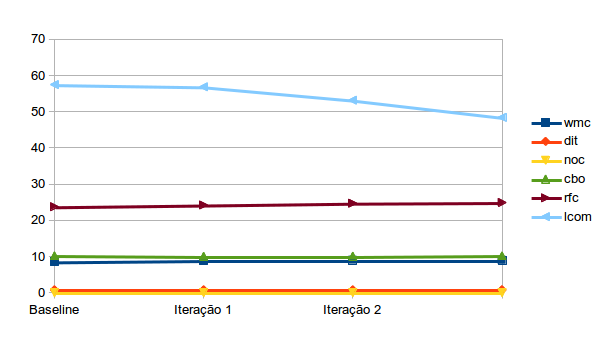
\includegraphics[scale=0.55]{img/allmetrics}
	\caption{\label{fig:allmetrics} Variação das métricas ao longo das iterações}
\end{figure}


É possível observar nos resutados a relação entre LCOM e as métricas 
WMC,RFC que aumentaram conforme o LCOM diminuia. O aumento da complexidade
indicado pelas métricas WMC e RFC é pequeno em comparação ao aumento de
coesão indicada pela métrica LCOM. Pode-se chegar a essa conclusão, não somente
analisando os resultados, como também ao analisar o código em que as classes
estão menores, mais coesas, com responsabilidades bem definidas. Portanto, a
arquitetura proposta melhorou a qualidade do objeto de estudo porque promoveu
maior coesão e diminuiu a complexidade.

\section{Conclusão} 

O presente trabalho avaliou os padrões de projetos Model View Controller e o
Model View Presenter mostrando em que contextos cada um se aplica para o
desenvolvimento da camada de apresentação de um sistema.
O padrão MVP define melhor as responsabilidades dos componentes para
implementação de interfaces levando em consideração os modelo de programação
usado no framework android onde as responsabilidades do Controller(definidos no
padrão MVC) estão implementadas nos próprios componentes visuais.

O padrão MVP foi implementado usando a variação chamada Passive View onde o
Model fica totalmente isolado da View. Esta variante foi usada pois evitou-se
fazer alterações em classes correspondentes a camada de Model, devido ao alto
acoplamento e grande complexidade do aplicativo, dessa forma foi possível evitar
que a refatoração gerasse algum erro no aplicativo, mantendo-o funcional. A
maioria das altreções estão presentes nas classes criadas para exercerem o papel
de Presenter.

As classes de View selecionadas para a refatoração extendem a classe Fragment.
A classe Fragment é usada para criar agrupamentos de componentes visuais que
possam ser reutilizados em outras partes do aplicativo. O uso da classe
Fragment foi mantido e parte das implementações presentes nessas classes foram
delegadas para as classes de Presenter correspondentes.

As métricas descritas por \cite{cksuite} foram usadas para avaliar os
impactos na qualidade do aplicativo após a refatoração usanddo o padrão MVP. Foi
usado o projeto CKJM para coletar os dados para fazer a análise.

Conforme um software é desenvolvido, novas classes e troca de mensagens são
implementadas afetando negativamente as métricas WMC, RFC e CBO. Não é possível
relacionar diretamente a métrica CBO com base na variação dos resultados para
esta métrica, apesar de que, os valore se mantiveram abaixo dos encontrados da
versão de referência, isso requer mais estudos abordando outros padrões de projeto.

%OK
A maioria das métricas tendem a aumentar durante o processo de refatoração. 
É válido resaltar que as três classes refatoradas são as mais complexas do
pacote de grupos com valores anômalos para as métricas. Portanto, somente após
uma refatoração em uma amostragem maior de classes que se é possível determinar
um valor de referência para as métricas, inclusive para um projeto construído
do zero. Com os dados coletados durante o desenvolvimento é possível definir
esses valores limites para identificar anomalias nas classes e tratar cada caso
isolado.

 
%\subsection{Trabalhos Futuros}

%Existem outros padrões de projetos para o desenvolvimento da camada de
%apresentação de um software que não foram analisados nesse trabalho, a saber: 
%MVVM, MVP-VM, MVPC. Essas variações no padrão MVC surgiram em contextos
%diversificados e podem agregar algum benefício à qualidade do aplicativo.
%Este trabalho não aborda o impacto do padrão MVP em outras métricas de
% qualidade de código derivadas do CK.
%Não foi feita uma avaliação dos impactos na performance do aplicativo devido ao
%uso do padrão MVP. A inclusão de mais objetos interagindo trocando mensagens
%pode depreciar a performance, levando-se em consideração sua execução em
%ambientes mais restritos, como no caso de um aparelho móvel.



% IEEEtran.cls defaults to using nonbold math in the Abstract.
% This preserves the distinction between vectors and scalars. However,
% if the conference you are submitting to favors bold math in the abstract,
% then you can use LaTeX's standard command \boldmath at the very start
% of the abstract to achieve this. Many IEEE journals/conferences frown on
% math in the abstract anyway.

% no keywords




% For peer review papers, you can put extra information on the cover
% page as needed:
% \ifCLASSOPTIONpeerreview
% \begin{center} \bfseries EDICS Category: 3-BBND \end{center}
% \fi
%
% For peerreview papers, this IEEEtran command inserts a page break and
% creates the second title. It will be ignored for other modes.
%\IEEEpeerreviewmaketitle








% trigger a \newpage just before the given reference
% number - used to balance the columns on the last page
% adjust value as needed - may need to be readjusted if
% the document is modified later
%\IEEEtriggeratref{8}
% The "triggered" command can be changed if desired:
%\IEEEtriggercmd{\enlargethispage{-5in}}

% references section

% can use a bibliography generated by BibTeX as a .bbl file
% BibTeX documentation can be easily obtained at:
% http://www.ctan.org/tex-archive/biblio/bibtex/contrib/doc/
% The IEEEtran BibTeX style support page is at:
% http://www.michaelshell.org/tex/ieeetran/bibtex/
\bibliographystyle{IEEEtran}
% argument is your BibTeX string definitions and bibliography database(s)
\bibliography{IEEE}
%
% <OR> manually copy in the resultant .bbl file
% set second argument of \begin to the number of references
% (used to reserve space for the reference number labels box)





% that's all folks
\end{document}


